% Clase del documento
\documentclass[12pt,twoside,titlepage]{report}





%%%%%%%%%%%%%%%%%%%%%%% Paquetes %%%%%%%%%%%%%%%%%%%%%%%

\usepackage[a4paper,bindingoffset=3mm,bottom=35mm]{geometry}


% Usad \usepackage[dvips]{graphicx} o \usepackage[pdftex]{graphicx} (no ambos)
%\usepackage[dvips]{graphicx} %%% para LaTeX. Las figuras deben estar en formato eps

\usepackage[colorlinks=true,pdftex]{hyperref}   %%% Opcional. Para incluir marcadores y enlaces en el pdf
\usepackage[pdftex]{graphicx}  %%% para pdflatex. Las figuras pueden estar en pdf, jpg, svg y otros formatos


\usepackage[spanish]{babel}

%\usepackage[latin1]{inputenc} % Usad en WinEdt/MikTex
\usepackage[utf8]{inputenc} % Usad en overleaf

%\usepackage[T1]{fontenc}


% Algunos paquetes útiles

\usepackage{amsmath,amssymb}
\usepackage{hyperref}
\usepackage{xcolor}
\usepackage{afterpage}
\usepackage{paralist}
\usepackage{array}
\usepackage{enumerate}
\usepackage{paralist}
\usepackage{enumitem}
\usepackage{float}
\usepackage{setspace}
\usepackage{listings}
\usepackage{algorithm}
\usepackage{algorithmic}
\usepackage{fancyhdr}
\usepackage{rotating}
\usepackage{multirow}
\usepackage{animate}
\usepackage{movie15}
\usepackage{media9}
\usepackage{graphicx}
\usepackage{epstopdf}
\usepackage{attachfile}
\usepackage{embedfile}
\usepackage{hypgotoe}

% Otros paquetes

\usepackage{quotchap}
\usepackage{lipsum}

%%%%%%%%%%%%%%%%%%%%%%%%%%%%%%%%%%%%%%%%%%%%%%%%%%%%%%%%

%%%%%%%%%%%%%%%%%%%%%%% Definiciones básicas %%%%%%%%%%%%%%%%%%%%%%%

\newcommand{\nombreautor}{Ángel Baeza Sánchez}
\newcommand{\nombretutor}{Aarón Sújar Garrido}
\newcommand{\titulotrabajo}{Herramienta de Prototipado de Videojuegos Plug \& Play}
\newcommand{\escuela}{Escuela Técnica Superior\\de Ingeniería Informática}
\newcommand{\escuelalargo}{Escuela Técnica Superior de Ingeniería Informática}
\newcommand{\universidad}{Universidad Rey Juan Carlos}
\newcommand{\fecha}{Fecha}
\newcommand{\grado}{Grado en Ingeniería de Computadores}
\newcommand{\curso}{Curso 2024-2025}
\newcommand{\logoUniversidad}{logoURJC.pdf} % logoURJC.eps

%%%%%%%%%%%%%%%%%%%%%%%%%%%%%%%%%%%%%%%%%%%%%%%%%%%%%%%%%%%%%%%%%%%%






%%%%%%%%%%%%%%%%%%%%%%%%% Otras definiciones %%%%%%%%%%%%%%%%%%%%%%%%%%

% Definiciones de colores (para hidelinks)
\definecolor{BlueLink}{rgb}{0.165,0.322,0.745}
\definecolor{PinkLink}{rgb}{0.8,0.22,0.5}
\definecolor{gray}{rgb}{0.6,0.6,0.6}


% Enlaces
\hypersetup{hidelinks,pageanchor=true,colorlinks,citecolor=PinkLink,urlcolor=black,linkcolor=BlueLink}


\newcommand\blankpage{%
    \newpage
    \null
    \thispagestyle{empty}%
    %\addtocounter{page}{-1}%
    \newpage}


% Texto referencias
\addto{\captionsspanish}{\renewcommand{\bibname}{Bibliografía}}

% Texto Índice de tablas
\addto\captionsspanish{
\def\tablename{Tabla}
\def\listtablename{\'{I}ndice de tablas}
}


\floatname{algorithm}{Algoritmo}

\newfloat{algorithm}{t}{lop}

%% Etiquetas de comentarios (tutor/alumno)
\newif\ifdraft
\drafttrue
\usepackage{subcaption}
\newcommand{\nb}[2]{
	{
		{\color{black}{
				\small\fbox{\bfseries\sffamily\scriptsize#1}
				{\sffamily\small$\triangleright~${\it\sffamily\small #2}$~\triangleleft$}
	}}}
}

\ifdraft
\newcommand\tutor[1]{\nb{Tutor}{\color{red}#1}}
\newcommand\alumno[1]{\nb{Alumno}{\color{blue}#1}}
\newcommand\cotutor[1]{\nb{Co-tutor}{\color{green}#1}}
\newcommand{\fixme}[1]{{\textcolor{red}{[FIXME] #1}}\xspace}
\newcommand{\cn}{{\color{violet}[citation required]}}

\else
%\usepackage[disable]{todonotes}
\newcommand\tutor[1]{}
\newcommand\alumno[1]{}
\newcommand\cotutor[1]{}
\newcommand{\fixme}[1]{}
\newcommand{\cn}{}

\fi






%\newenvironment{pseudocodigo}[1][htb]
%  {\renewcommand{\algorithmcfname}{Pseudocódig}% Update algorithm name
%   \begin{algorithm}[#1]%
%  }{\end{algorithm}}
  
%%%%%%%%%%%%%%%%%%%%%%%%%%%%%%%%%%%%%%%%%%%%%%%%%%%%%%%%%%%%%%%%%%%%





%%%%%%%%%%%%%%%%%%%%%%% Estilo de código (en Python) %%%%%%%%%%%%%%%%%%%%%%%

\definecolor{bg}{rgb}{0.95,0.95,0.95}
\definecolor{mydeepteal}{rgb}{0.16,0.22,0.23}
\definecolor{myteal}{rgb}{0.31,0.44,0.46}
\definecolor{mymediumteal}{rgb}{0.41,0.58,0.60}

\DeclareFixedFont{\ttb}{T1}{txtt}{bx}{n}{12} % for bold
\DeclareFixedFont{\ttm}{T1}{txtt}{m}{n}{12}  % for normal


%\newcommand*{\FormatDigit}[1]{\textcolor{mydeepteal}{#1}}
\newcommand*{\FormatDigit}[1]{\textcolor{black}{#1}}

% Python style for highlighting
\newcommand\mypythonstyle{\lstset{
language=Python,
basicstyle=\ttfamily\small,
%basicstyle=\linespread{1.0}\footnotesize\ttm,
otherkeywords={self},             % Add keywords here
keywordstyle=\bfseries\ttfamily\color{myteal},
%keywordstyle=\ttb\color{myteal},
commentstyle=\itshape\color{myteal},
stringstyle=\color{mydeepteal},
emph={MyClass,__init__},          % Custom highlighting
emphstyle=\ttb\color{mydeepteal},    % Custom highlighting style
% Any extra options here
showstringspaces=false,            %
backgroundcolor=\color{bg},
rulecolor = \color{bg},
%identifierstyle=\color{deepgreen},
breaklines=true,
numbers=left,
numbersep=5pt,
numberstyle=\tiny,
tabsize=4,
xleftmargin=1em,
frame = single,
framesep = 3pt,
framextopmargin=0pt,
framexbottommargin=0pt,
framexleftmargin=0pt,
framexrightmargin=0pt,
fontadjust=true,
basewidth=0.55em, % compactness of code
upquote=true,
}}

% Python environment
\lstnewenvironment{mypython}[1][]
{
\mypythonstyle
\lstset{#1}
}
{}

\newcommand\mypythonstylenormalinline{\lstset{
language=Python,
basicstyle=\ttfamily\normalsize,
%basicstyle=\linespread{1.0}\footnotesize\ttm,
otherkeywords={self},            % Add keywords here
keywordstyle=\bfseries\ttfamily\color{myteal},
%keywordstyle=\ttb\color{myteal},
commentstyle=\itshape\color{mymediumteal},
stringstyle=\color{mydeepteal},
emph={MyClass,__init__},          % Custom highlighting
emphstyle=\ttb\color{mydeepteal},    % Custom highlighting style
% Any extra options here
showstringspaces=false,            %
backgroundcolor=\color{bg},
rulecolor = \color{bg},
%identifierstyle=\color{deepgreen},
breaklines=false,
numbers=left,
numbersep=5pt,
numberstyle=\tiny,
tabsize=4,
xleftmargin=0em,
frame = single,
framesep = 3pt,
framextopmargin=0pt,
framexbottommargin=0pt,
framexleftmargin=0pt,
framexrightmargin=0pt,
fontadjust=true,
%basewidth=0.55em, % compactness of code
upquote=true,
}}

\newcommand\mypythoninline[1]{{\mypythonstylenormalinline\lstinline!#1!}}

%%%%%%%%%%%%%%%%%%%%%%%%%%%%%%%%%%%%%%%%%%%%%%%%%%%%%%%%%%%%%%%%%%%%%%%%%%%%%%




%%%%%%%%%%%%%%%%%%%%%%%%%%%% Comandos definidos por el autor 

\newcommand{\transpuesta}{\mbox{\tiny $\mathsf{T}$}}








%%%%%%%%%%%%%%%%%%%%%%%%%%%%%%%%%%%%%%%%%%%%%%%%%%%%%%%%%%%%%%%%%%%%%%%
%                           Inicio del documento                       
%%%%%%%%%%%%%%%%%%%%%%%%%%%%%%%%%%%%%%%%%%%%%%%%%%%%%%%%%%%%%%%%%%%%%%%

\newcommand*{\embedfileandcreatelink}[2]{\embedfile{#1}\href{gotoe:embedded=#1}{#2}}

\begin{document}

\pagestyle{plain}




%%%%%%%%%%%%%%%%%%%%%%%%%%%%%%%%%%%% Portada %%%%%%%%%%%%%%%%%%%%%%%%%%%%%%%%%%

%\pagenumbering{gobble}
%\pagenumbering{arabic}

% Universidad, Facultad
\begin{titlepage}
\selectlanguage{spanish}


% logo
\begin{center}
    \includegraphics[scale=0.7]{\logoUniversidad}
\end{center}

\bigskip

\begin{center}
\begin{LARGE}
\escuela \\
\end{LARGE}
\end{center}

\bigskip
\bigskip

% Grado
\begin{center}
\begin{large}
\textbf{\grado}\\
\end{large}
\end{center}

% Curso
\begin{center}
\begin{large}
\textbf{\curso}\\
\end{large}
\end{center}

\bigskip

\textbf{\begin{center}
\begin{large}
\textbf{Trabajo Fin de Grado}
\end{large}
\end{center}}

\bigskip
\bigskip
\bigskip

% Nombre del TFG
\begin{center}
\textbf{\begin{large}
\MakeUppercase{\titulotrabajo}\\
\end{large}}
\end{center}

% Nombre del autor
\vspace{\fill}
\begin{center}
\textbf{Autor: \nombreautor}\\ \smallskip
% Tutor
\textbf{Tutor: \nombretutor}\\
% Añadir segundo tutor si hubiera


\bigskip

% Fecha
%\textbf{\fecha}\\
\end{center}
\end{titlepage}


%%%%%%%%%%%%%%%%%%%%%%%% Opcional %%%%%%%%%%%%%%%%%%%%%%
%\blankpage

%\thispagestyle{empty}
%\begin{center}

% Nombre del trabajo
%\textbf{\begin{large}
%\MakeUppercase{\titulotrabajo}\\*
%\end{large}}
%\vspace*{0.2cm}
%\vspace{5cm}

% Nombre del autor y del tutor
%\large Autor: \nombreautor \\* \medskip
%\large Tutor: \nombretutor \\*

%\vfill

% Escuela, universidad y fecha
%\escuelalargo \\ \smallskip
%\universidad \\
%\vspace{1cm}
%\fecha \\

%\clearpage

%\end{center}
%%%%%%%%%%%%%%%%%%%%%%%%%%%%%%%%%%%%%%%%%%%%%%%%%%%%%%%%

\hypersetup{pageanchor=true}

\normalsize
\afterpage{\blankpage} % Se deben añadir página en blanco para que lo capítulos de la memoria o estas secciones introductorias empiecen en páginas impares

%%%%%%%%%%%%%%%%%%%%%%%%%%%%%%%%%%%%%%%%%%%%%%%%%%%%%%%%%%%%%%%%%%%%%%%%%%%%%%%





% Estilo de párrafo de los capítulos
\setlength{\parskip}{0.75em}
\renewcommand{\baselinestretch}{1.25}
% Interlineado simple
\spacing{1}

\pagenumbering{Roman}
\setcounter{page}{2}


%%%%%%%%%%%%%%%%%%%%%%%%% Agradecimientos o dedicatoria %%%%%%%%%%%%%%%%%%%%%%%%%%%

\chapter*{Agradecimientos}

Quisiera agradecer a mis padres y a mi hermana, por su apoyo incondicional durante toda mi vida, también por su excelente sentido del humor, sin el cuál no creo que hubiera llegado (vivo) a donde estoy hoy.

También a mi pareja, Eva, por estar siempre a mi lado pase lo que pase, por su apoyo y cariño infinitos en los mejores y peores días y por soportarme estos últimos meses de estrés para terminar la carrera. Te quiero.

A mis compañeros de piso, Ceci, Javi y Vicente por ser una segunda familia, y por su ayuda constante en mi día a día, sois amigos increíbles.

Y finalmente a mis amigos del grado, sin los cuales no me habría sacado ni el primer examen de primero de carrera, muchas gracias por contestar esas dudas incesantes los veinte minutos antes de cada examen.


\afterpage{\blankpage}

%%%%%%%%%%%%%%%%%%%%%%%%%%%%%%%%%%%%%%%%%%%%%%%%%%%%%%%%%%%%%%%%%%%%%%%%%%%%%%%%%%%






%%%%%%%%%%%%%%%%%%%%%%%%%%%%%%%%%%%% Resumen %%%%%%%%%%%%%%%%%%%%%%%%%%%%%%%%%%%%%%

\chapter*{Resumen}

El desarrollo de videojuegos es un proceso arduo y complejo, en el que una gran variedad de disciplinas se entrelazan para crear una obra simultáneamente artística y técnica.
 Con el fin de hacer que este tipo de proyectos sean más abarcables una gran parte de la industria se sustenta sobre distintas herramientas cuya única función es agilizar 
 los distintos procesos que forman parte de esta.

Este proyecto es una de dichas herramientas, cuyo objetivo es proporcionar una serie de mecánicas y sistemas ampliables y modulares que permitan agilizar tanto la fase de
 prototipado como ciertas partes del desarrollo que tienden a ser muy parecidas, sino idénticas en la mayoría de videojuegos.

En este documento se detallan una descripción en profundidad de: motivaciones, objetivos, análisis de requisitos, validación y conclusiones en lo relativo al proyecto.
 Además de un análisis técnico en profundidad de los distintos módulos del proyecto.

\mbox{} \bigskip

\noindent \textbf{Palabras clave}:
\begin{compactitem}
    \item Unity
    \item Sistemas de diálogo
    \item Laberintos
    \item Mazmorras
    \item Desarrollo de Videojuegos
    \item Herramientas de Desarrollo de Videojuegos
    \item C\#
\end{compactitem}


\chapter*{Abstract}

Videogame development is an arduous and complex process, in which a great variety of disciplines intertwine to create titles which are both artistic and technical wonders.
 As a means to make these types of projects somewhat less incommensuralbe, a big part of the industry is sustained by several different tools whose only purpose is to streamline the different processes that are part of it.  

This project is one of such tools, whose objective is to provide a series of mechanics and modular systems that aim to improve both the prototyping phase as well as some parts
 of development which tend to be similar, if not identical in the majority of videogames.

This document contains an in depth description of the: motivations, objectives, requirement analysis, validation and conclusions pertaining this project. As well as an in
 depth technical analysis of the different modules by which the project is composed.

\mbox{} \bigskip

\noindent \textbf{Keywords}:
\begin{compactitem}
    \item Unity
    \item Dialogue Systems
    \item Labyrinths
    \item Dungeons 
    \item Videogame Development
    \item Videogame Development Tools
    \item C\#
\end{compactitem}


\afterpage{\blankpage}


%%%%%%%%%%%%%%%%%%%%%%%%%%%%%%%%%%%%%%%%%%%%%%%%%%%%%%%%%%%%%%%%%%%%%%%%%%%%%%%%%%%





%%%%%%%%%%%%%%%%%%%%%%%%%%%%%%%%%%%% Índices %%%%%%%%%%%%%%%%%%%%%%%%%%%%%%%%%%%%

% Estilo de párrafo de los Índices
\setlength{\parskip}{1pt}
\renewcommand{\baselinestretch}{1}
\renewcommand{\contentsname}{Índice de contenidos}


% Índice de contenidos
\tableofcontents
\afterpage{\blankpage}

% Índice de tablas (OPCIONAL)
\listoftables
\addcontentsline{toc}{chapter}{\noindent \listtablename}

% Índice de figuras (OPCIONAL)
\listoffigures
\addcontentsline{toc}{chapter}{\listfigurename}

% Índice de códigos/algoritmos (OPCIONAL).   El término "Códigos" se puede cambiar por "Métodos", "Funciones", "Algoritmos", etc.
\renewcommand\lstlistlistingname{Códigos}
\renewcommand\lstlistingname{Código}
\renewcommand\lstlistlistingname{Índice de códigos}

\lstlistoflistings
\addcontentsline{toc}{chapter}{\lstlistlistingname}


% En este documento (de momento) no se ha considerado incluir un índice de algoritmos/pseudocódigos, como el que aparece en \ref{AdditionalLouvain}

%%%%%%%%%%%%%%%%%%%%%%%%%%%%%%%%%%%%%%%%%%%%%%%%%%%%%%%%%%%%%%%%%%%%%%%%%%%%%%%%%%%





%%%%%%%%%%%%%%%%%%%%%%% Cabeceras y pies de página (Opcional) %%%%%%%%%%%%%%%%%%%%%%%

%\setlength{\headheight}{15.2pt}
\pagestyle{fancy}


\renewcommand{\chaptermark}[1]{\markboth{Capítulo \thechapter.\ #1}{}}

\pagestyle{fancy}
\fancyhf{}
\fancyhead[LO]{\leftmark}
\fancyhead[RO]{}
\fancyhead[RE]{\nouppercase\rightmark}
\fancyhead[LE]{}
\fancyfoot[C]{\thepage}

%%%%%%%%%%%%%%%%%%%%%%%%%%%%%%%%%%%%%%%%%%%%%%%%%%%%%%%%%%%%%%%%%%%%%%%%%%%%%%%%%%%%






%%%%%%%%%%%%%%%%%%%%%%%%%%%%%% Capítulos de la memoria %%%%%%%%%%%%%%%%%%%%%%%%%%%%%



% Capítulo 1
\chapter{Introducción}
\label{sec:intro}


%%%%%%%%%%%%%%%%%%%%%%%%%%%%%%%%%%%%%%%%%%%%%%%%%%%%%%%%%%%%%%%%%%%%%%%%%%

% Estilo resto de páginas
\pagestyle{fancy}


% Estilo de párrafo de los capítulos
\setlength{\parskip}{0.75em}
\renewcommand{\baselinestretch}{1.25}
% Interlineado simple
\spacing{1}
% Numeración contenido
\pagenumbering{arabic}
\setcounter{page}{1}

%%%%%%%%%%%%%%%%%%%%%%%%%%%%%%%%%%%%%%%%%%%%%%%%%%%%%%%%%%%%%%%%%%%%%%%%%%

\section{Descripción General}
En este documento se desarrollarán las motivaciones, implicaciones y detalles de la implementación de este Trabajo de Fin de Grado.

El objetivo general de este proyecto ha sido el desarrollo de un paquete de herramientas y sistemas modulares que permitan agilizar el proceso de desarrollo de un videojuego. 
El paquete está compuesto de cinco módulos distintos, que a su vez se componen de una serie de herramientas o sistemas con diversas funciones, también incluye una serie de 
escenas de prueba en las que se pueden ver los diversos sistemas en acción. Además, cada módulo y submódulo incluye todos los 'prefabs' necesarios para su funcionamiento 
inmediato. 

Los distintos módulos son: 
\begin{compactitem}
  \item Sistemas Atómicos.   
  \item Herramientas de Debug
  \item Generador de Mazmorras
  \item Componentes Independientes de Unity
  \item Componentes de Movimiento de Personajes
\end{compactitem} 
\subsection{Sistemas Atómicos}
El módulo de Sistemas Atómicos está compuesto por los siguientes submódulos:
\begin{itemize}
  \item Sistema de Diálogos: Incluye un editor de diálogos basado en grafos que permite esquematizar flujos conversacionales con distintas respuestas posibles, 
  además de exportarlo a un formato legible por otra herramienta de editor que permite colocar dichos diálogos en el nivel, con distintos tipos de desencadenantes. Además, 
  el sistema incluye una implementación de efectos de texto modular que permite añadir animaciones al texto basándose en los vértices del mallado. 
  \item Sistema de Experiencia: Es un sencillo sistema que permite definir una serie de constantes para personalizar un sistema de niveles para habilidades o personajes,
   además de poder elegir entre una serie de algoritmos para definir la curva de adquisición de experiencia. 
  \item Sistema de audio: Permite la definición de distintas canciones y sonidos como Scriptable Objects y reproducirlos en distintos canales de audio 
   mediante la invocación de funciones estáticas.
  \item Sistema de guardado: Trae una serie de funciones utilitarias que permite guardar cualquier variable alfanumérica, lista o mapa en formato JSON en el directorio 
   especificado, además de permitir encriptar dicho fichero. Este sistema trae también una implementación para varias ranuras de guardado, funciones para crear, copiar y
   eliminar ranuras de guardado.
  \item Sistema de Gestión de Carga de Escenas: Un paquete que se compone de distintas funciones que permiten cargar escenas de forma asíncrona, descargando automáticamente 
   la escena actual y permitiendo definir una pantalla de carga intermedia para hacer la transición más agradable.
\end{itemize}

\subsection{Herramientas de Debug}
Las herramientas de debug son sencillos scripts que tienen como objetivo hacer que la depuración de errores sea más cómoda, este paquete incluye:
\begin{compactitem}
  \item Componente de Dibujado de Colisiones 2D: Consiste en un componente que dibuja las colisiones en la ventana de 'play' de Unity y en versiones empaquetadas.   
  \item Herramienta de cuadrícula : Consiste en un componente que se ejecuta solo en modo debug, y hace más sencillo colocar los elementos de la escena siguiendo una
   cuadrícula de un tamaño especificado en el inspector del componente. 
\end{compactitem} 

\subsection{Generador de Mazmorras}
El generador de Mazmorras es una herramienta que utiliza una serie de algoritmos de recorrido de grafos para generar laberintos o mazmorras, e incluye una serie de clases
 utilitarias que permiten buscar el camino mínimo, convertir las estructuras de mazmorras/laberintos a grafos pesados o matrices.

\subsection{Componentes Independientes de Unity}
Este módulo contiene las características que son o bien una colección de funciones estáticas, sistemas simples contenidos en una sola clase o componentes de Unity 
 con funcionalidades sencillas.
\begin{compactitem}
  \item 'Floater': Sencillo script que hace que cualquier objeto de la escena flote siguiendo una función sinuidal. También hace que rote sobre sí mismo dada una velocidad.
  \item Componente de Vida: Permite asignar vida a un objeto y definir eventos que provocan una pérdida de vida o que reaccionen a ello. 
  \item Componente de Interacción: Permite añadir a un objeto una serie de eventos que se ejecuten cuando el jugador interactúe con el mismo. También permite definir un
   rango en el cual pueda interactuar. 
  \item 'LaunchRigidbody': Función estática que permite lanzar cualquier objeto con físicas con una dirección y fuerza específicas.
  \item 'LookAtCamera': Componente que provoca que el objeto que lo contenga siempre mire hacia cámara, útil para textos u objetos 2D de la escena.
  \item Componentes de Sacudida de Cámara: Sistema que, mediante funciones estáticas, permite sacudir cámaras de Unity o 'Cinemachine' en escenarios 2D y 3D, permite
   definir la intensidad de la sacudida basada en curvas de animación.
\end{compactitem}

\subsection{Componentes de Movimiento de Personajes}
Este módulo está compuesto por una colección de 'prefabs' que, con sus scripts asociados, permiten añadir a una escena un personaje jugable con unos controles y cámara asociados.
Todas las configuraciones posibles contienen tanto una implementación basada en movimiento discreto como otra basada en físicas, las diferentes configuraciones son: 
\begin{compactitem}
  \item 2D Lateral o 'Side Scroll': Permite jugar con un esquema de controles similar al de un plataformas clásico como 'Super Mario World' (Figura \ref{fig:smbw}).
  \item 2D Cenital o 'Top Down': Permite jugar con un esquema de controles similar al de el primer 'The Legend of Zelda' o 'Hotline Miami' (Figura \ref{fig:hlmiami}).
  \item 3D Primera Persona o 'First Person': Permite jugar con un esquema de controles similar a 'Doom' o 'Call of Duty' (Figura \ref{fig:doometernal}).
  \item 3D Tercera Persona o 'Third Person': Permite jugar con un esquema de controles similar a 'Grand Theft Auto', 'God of War: Ragnarok' o 'Blades of Fire' (Figura \ref{fig:bof}). Esta configuración permite escoger entre varios 
   tipos de posicionamiento de cámara para ese mismo esquema, como por ejemplo: tercera persona clásica , vista cenital, isométrica, o cámara al hombro. 
  \item 3D Lateral o 'Side Scroll': Permite jugar con un esquema de controles similar a 'Metroid Dread' (Figura \ref{fig:mdread}).
\end{compactitem}
\raggedbottom
\begin{figure}[H]
  \centering
    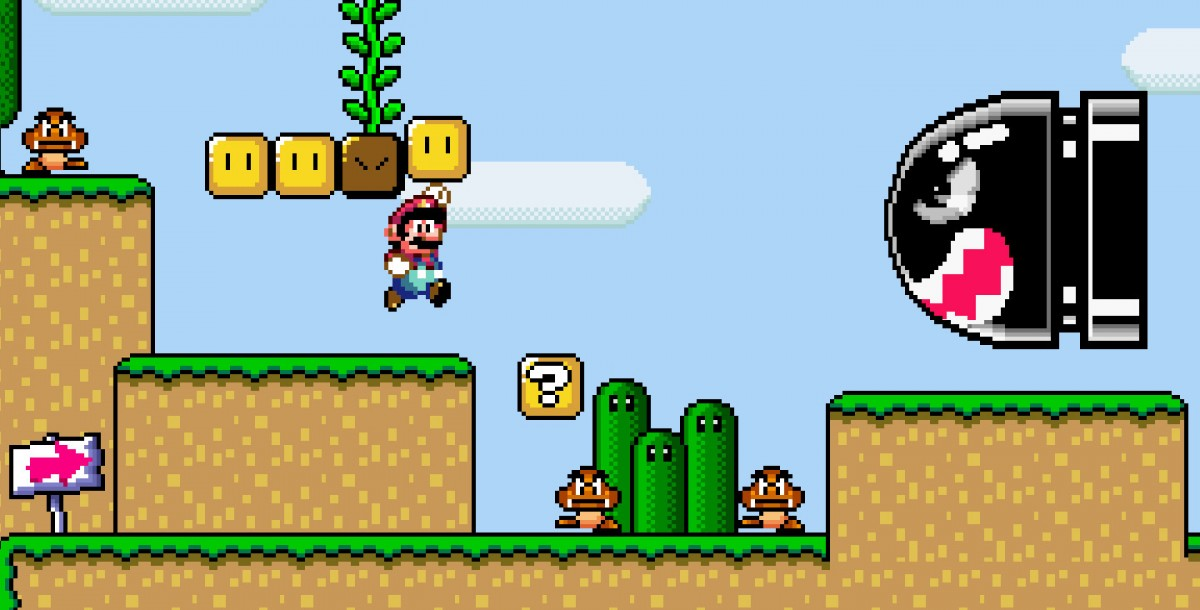
\includegraphics[width=350px,clip=true]{super_mario_world.jpg}
  \caption{2D side scroll, Super Mario World.}
  \label{fig:smbw}
\end{figure}

\begin{figure}[H]
  \centering
  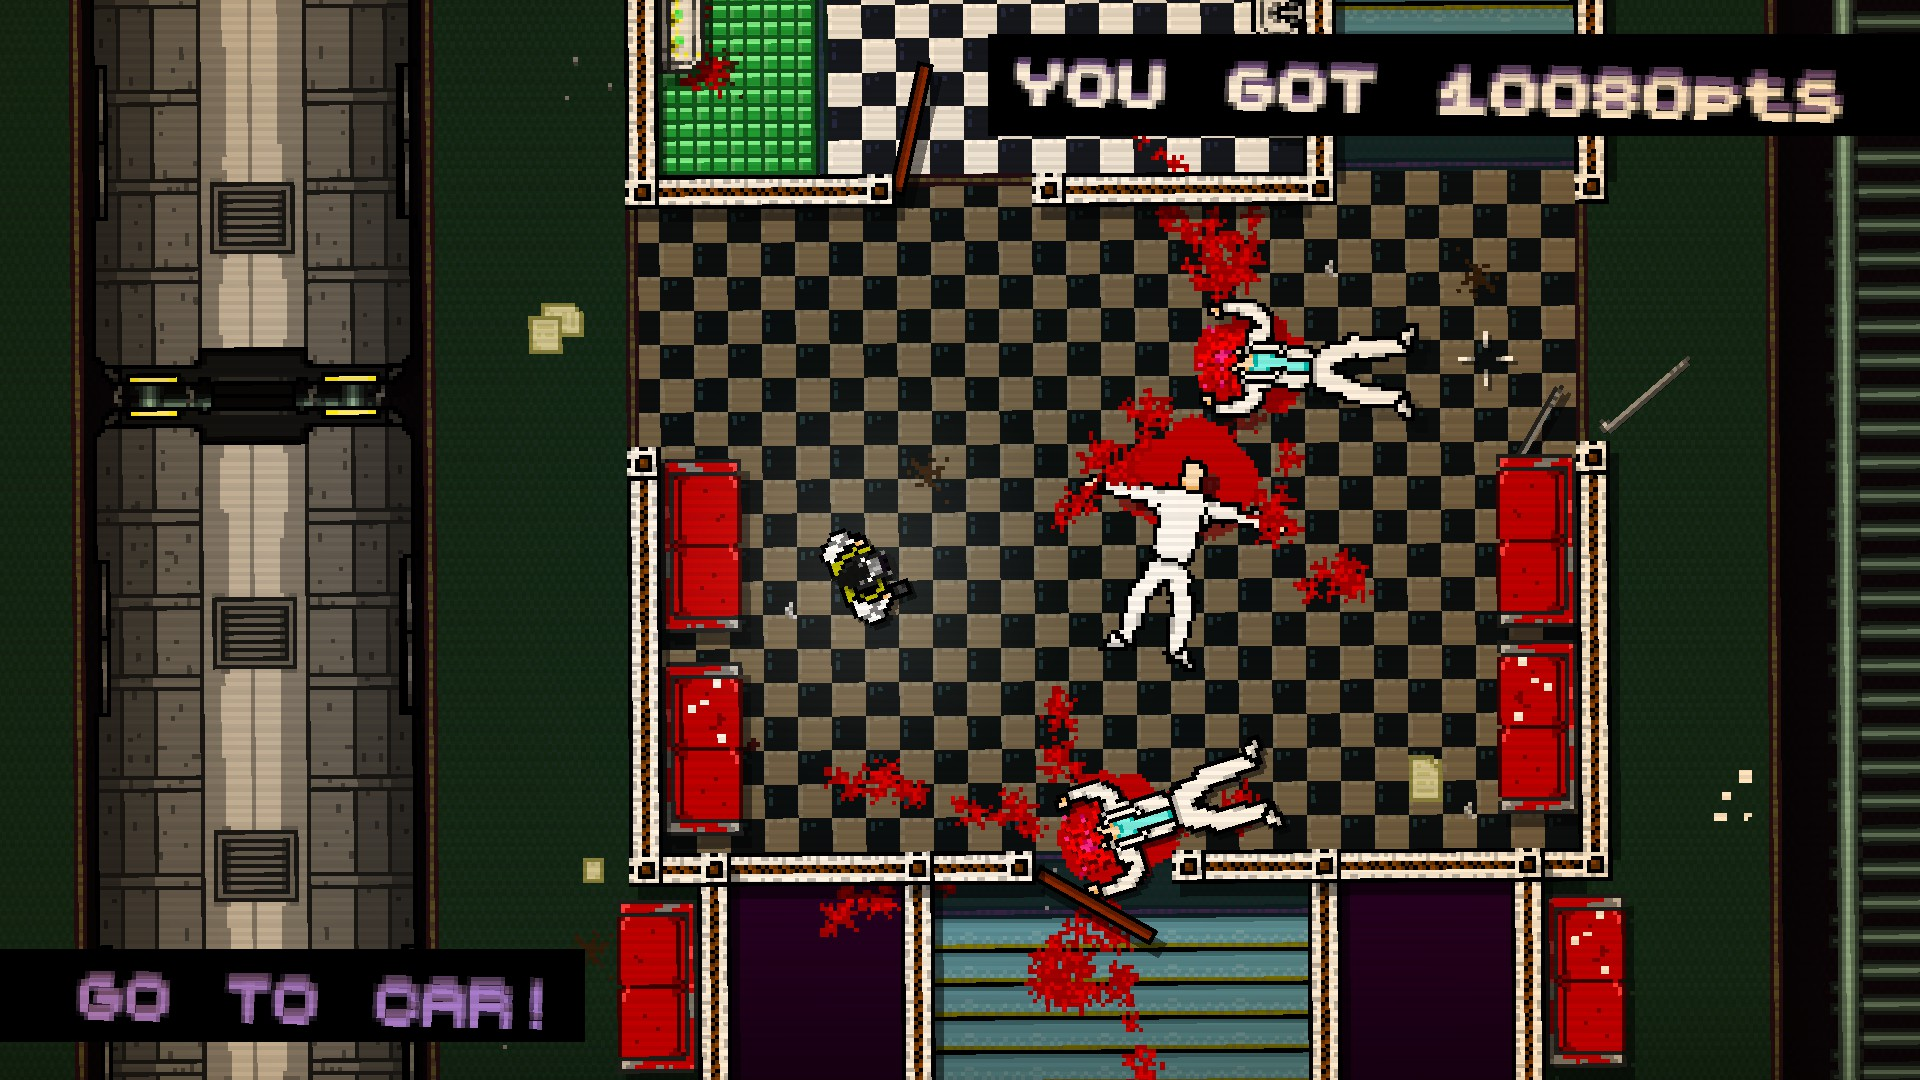
\includegraphics[width=350px,clip=true]{hotline_miami.png}
  \caption{2D top down, Hotline Miami.}
  \label{fig:hlmiami}
\end{figure}

\begin{figure}[H]
  \centering
  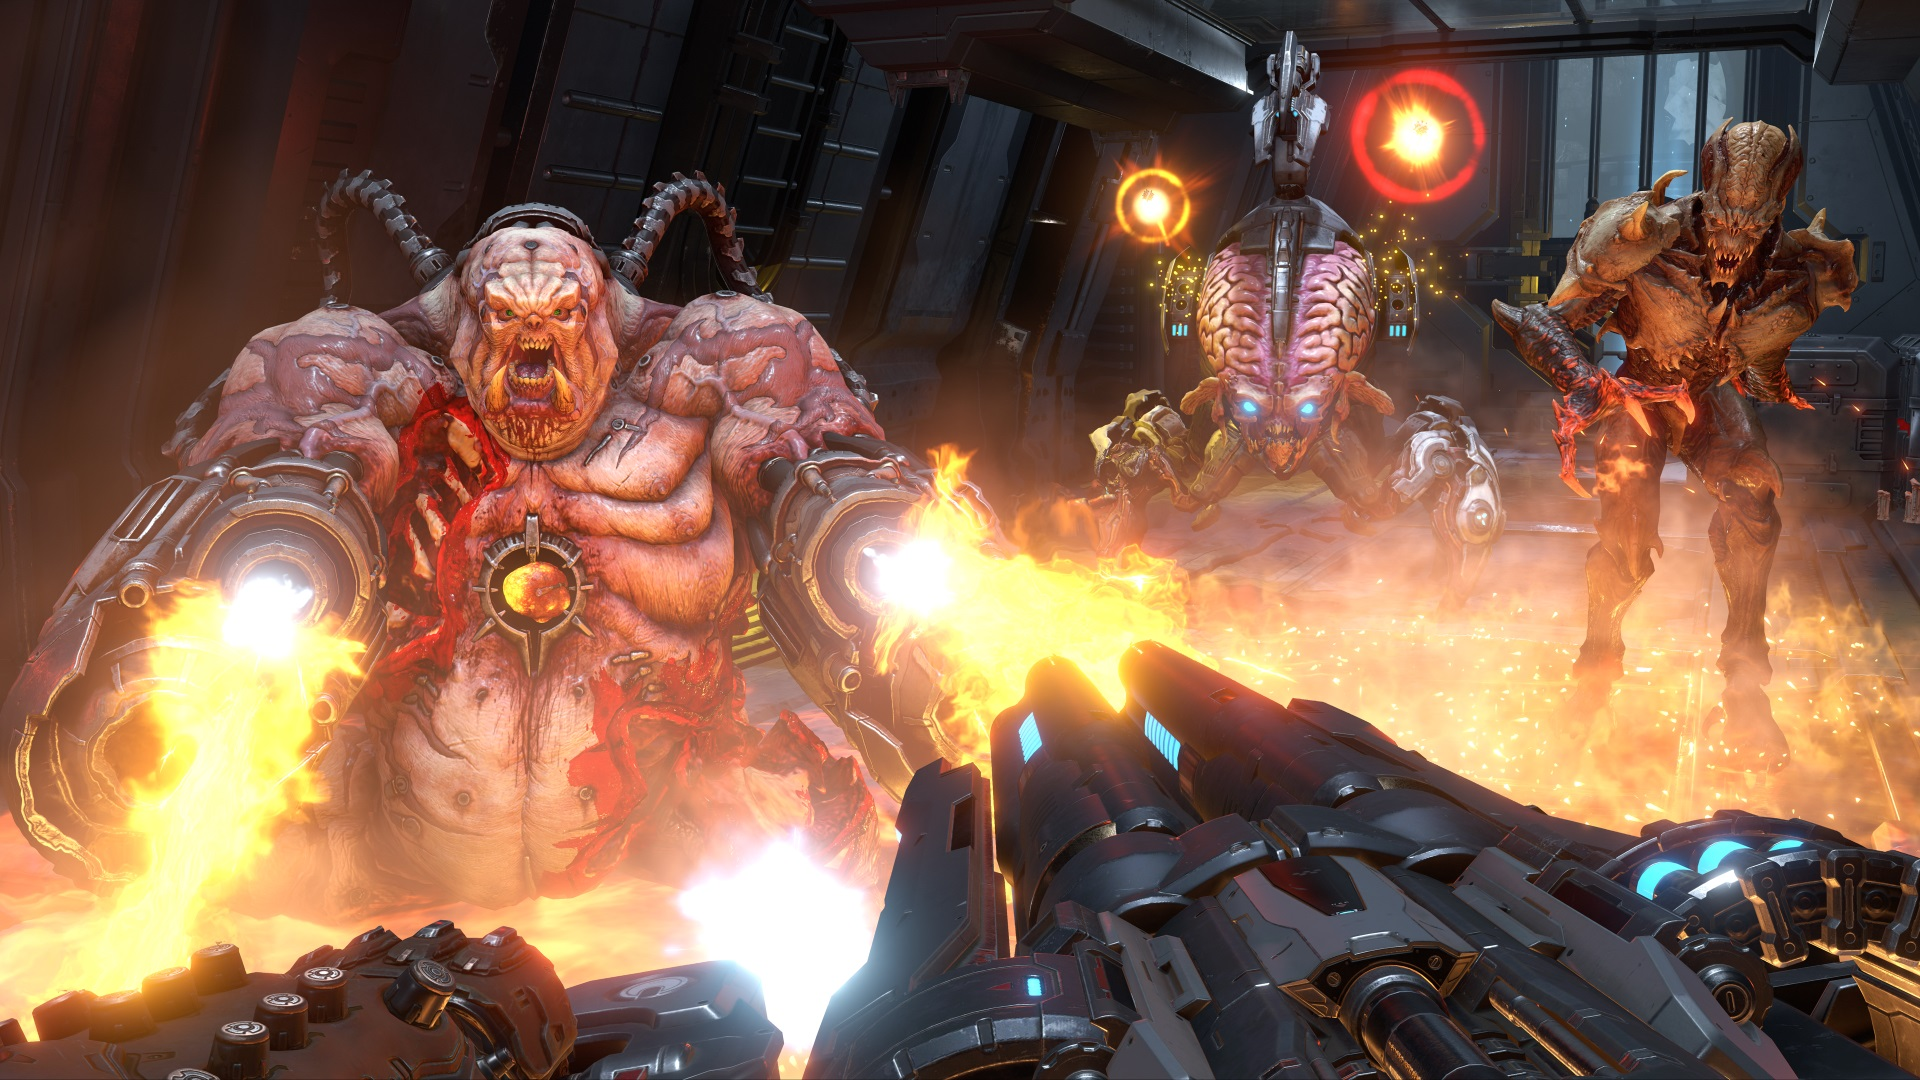
\includegraphics[width=350px,clip=true]{doom_eternal.png}
  \caption{3D primera persona, Doom Eternal.}
  \label{fig:doometernal}
\end{figure}

\begin{figure}[H]
  \centering
  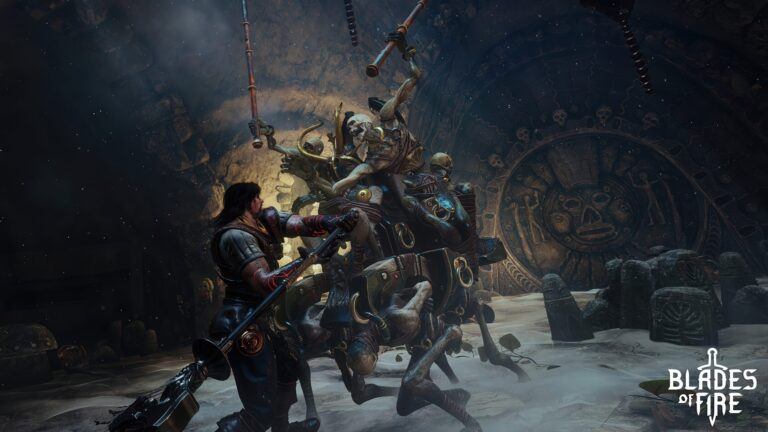
\includegraphics[width=350px,clip=true]{bof.png}
  \caption{3D tercera persona, Blades of Fire.}
  \label{fig:bof}
\end{figure}

\begin{figure}[H]
  \centering
  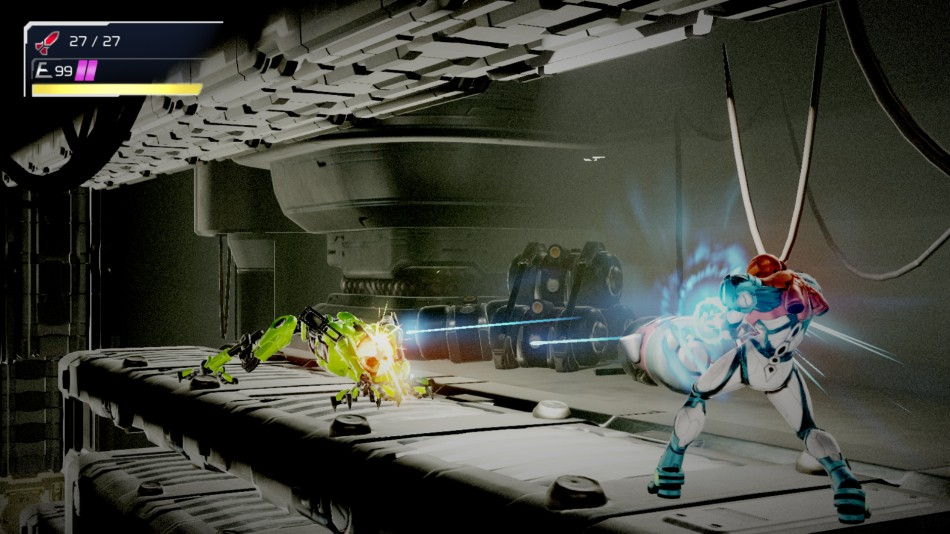
\includegraphics[width=350px,clip=true]{dread.png}
  \caption{3D side scroll, Metroid Dread.}
  \label{fig:mdread}
\end{figure}

\section{Motivación}

La motivación para el desarrollo de este proyecto ha sido la reiterada necesidad de una serie de funcionalidades básicas a lo largo de mi trayectoria como desarrollador,
 en trabajos de clase, participando en 'Game Jams' o en proyectos independientes. Pese a que algunas de las funcionalidades contenidas en el paquete ya existen en el mercado,
 se ha buscado en todos los casos aportar una solución más general, funcional y escalable que las alternativas disponibles. El resultado es un paquete que intenta proporcionar
 una 'suite' de herramientas que agilicen el prototipado de videojuegos, y permitan ampliar la funcionalidad base conforme el proyecto requiera de funciones más específicas. 
 Por tanto se puede extraer que tanto una motivación como un objetivo sería desarrollar una librería de funcionalidades que pueda asistir a equipos futuros a desarrollar
 videojuegos de forma más ágil.

Este enfoque tiene como objetivo que el paquete sea lo más transversal y usable posible para desarrolladores de todos los niveles (siempre y cuando tengan una formación básica).
 De forma que permite a desarrolladores sin mucha experiencia utilizar el paquete en su forma básica, la cual contiene suficiente funcionalidad como para poder crear juegos
 sencillos, además de permitir a desarrolladores más experimentados utilizar y evolucionar las herramientas para crear mecánicas y dinámicas complejas.
 
 Finalmente habría que considerar también la motivación adicional de aprender el uso de nuevas tecnologías mediante el desarrollo de un proyecto, que tendría como objetivo el
  propio aprendizaje y la acumulación de experiencia de llevar un proyecto desde su etapa de concepción hasta validarlo con el prototipado y finalización de un videojuego. 

%\raggedbottom
\section{Objetivos}
\subsection{Objetivos generales}
El objetivo general del trabajo es la elaboración de una librería completa y funcional con la los usuarios puedan prototipar videojuegos de forma ágil y sencilla. 
 En dicha librería deberían haber sistemas que permitan gestionar diálogos, archivos de guardado, sonido, niveles y cargas. Además de componentes independientes que permitan 
 el uso de físicas, movimiento y sacudida de cámara. Además, deberá incluir herramientas de depuración propias para auxiliar tanto las herramientas propias como las del motor. 
 Finalmente la 'suite' de herramientas deberá permitir la generación procedimental de laberintos y mazmorras.

\subsection{Escalabilidad}
El objetivo más importante del proyecto, por encima de implementar todas las características deseadas, es que todos los componentes queden bien documentados, sean funcionales
 y escalables. De forma que, como se ha mencionado anteriormente, usuarios con cualquier nivel de experiencia puedan hacer uso de las herramientas expuestas. De este modo, 
 además de pulir dichas herramientas, el código debe de estar implementado de forma que, ya sea mediante patrones, composición y/o herencia, se pueda ampliar la funcionalidad dispuesta
 cómodamente.
 
\subsection{Documentación}
Como consecuencia, para mantener un código limpio y escalable, es necesario escribir un documento detallando el modo de uso y funcionamiento de todas las características del paquete.

\subsection{Niveles de prueba}
Otro de los objetivos es construir niveles de prueba que puedan servir a los usuarios como tutoriales o ejemplos del uso de las herramientas incluidas en el paquete. Dichos 
 niveles deben estar bien organizados y etiquetados, y deben permitir a los usuarios entender como funcionan los componentes que habiten en ellos.

\subsection{Validación}

El paquete necesitará ser validado por usuarios reales, que utilicen las herramientas proporcionadas por el mismo para desarrollar un prototipo jugable, para conseguir esto,
 se prepararán al menos dos equipos que participarán en una 'Game Jam' y desarrollarán dicho prototipo disponiendo de las herramientas de la librería que crean convenientes.
 Al finalizar el evento, estos usuarios deberán rellenar una encuesta de satisfacción acerca de la librería, y se llevarán a cabo los ajustes que se puedan extrapolar de
 los resultados.  

\subsection{Resumen de Objetivos}

En resumen, el el proyecto pretende, como objetivo principal desarrollar un paquete de herramientas completo y funcional que permita a los usuarios prototipar y 
 desarrollar videojuegos. Dicho paquete debe contener diversos sistemas y componentes 'prefabricados' que agilicen el desarrollo. 

Además de los objetivos secundarios:
\begin{compactitem}
  \item Que los componentes del paquete sean escalables.
  \item Desarrollar niveles de prueba para servir a modo de tutorial para los usuarios.
  \item Documentar el modo de uso y funcionamiento de los componentes del proyecto.
  \item Validar el paquete con usuarios reales.
  \item Construir varios prototipos utilizando el paquete.
  \item Ajustar el paquete en base a los resultados de una encuesta de satisfacción.
\end{compactitem}

\section{Metodología}
Para el desarrollo de la librería se ha utilizado una metodología de trabajo en cascada, dado que el desarrollo lo ha llevado a cabo una única persona, lo cual
impide la paralelización de tareas que ofrece una metodología ágil. Sin embargo si que se han tenido en cuenta ciertos elementos de la metodología Agile, como 
por ejemplo utilizar un tablón de tareas con estados de 'To Do', 'Doing' y 'Done' con algunas modificaciones (Figura \ref{fig:trello}).

\begin{figure}[H]
  \centering
	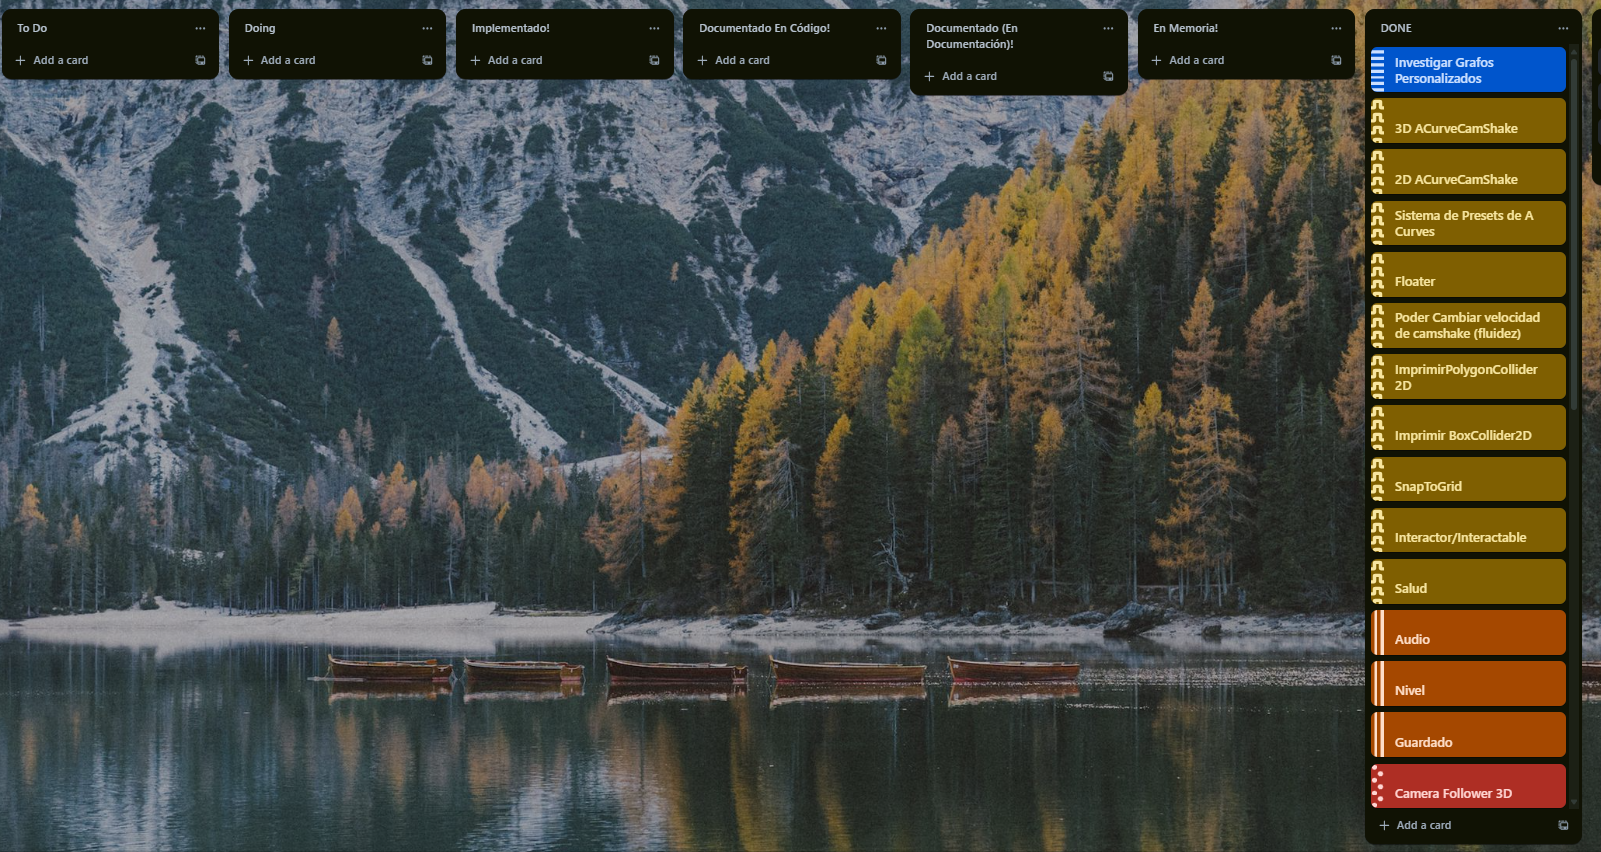
\includegraphics[width=350px,clip=true]{trello2.png}
  \caption{Tablero de Trello en imitación a la metodología Agile, con pasos extra para identificar el proceso de documentación,}
  \label{fig:trello}
\end{figure}

El desarrollo se puede dividir en tres fases: 
\begin{itemize}
	\item Fase 1: Pre-Producción y Análisis de Requisitos, Junio 2024 - Diciembre 2024
	\item Fase 2: Producción, Enero 2025 - Mayo 2025
	\item Fase 3: Polish, Desarrollo de Niveles de Prueba, Documentación y Validación, Junio 2025
\end{itemize}

La primera fase se utilizó como una ventana de tiempo en la que prototipar los componentes más completos, como el sistema de diálogo o la generación de
 mazmorras. También se dedicó a desarrollar un análisis de requisitos en los que definir que herramientas y componentes se iban a desarrollar. 
 
Durante la segunda fase se realizó el groso de la producción de la librería, con un análisis de requisitos sólido, esta fase consistió en la implementación y testeo 
finales de los componentes más complejos, así como la totalidad del desarrollo de los componentes más sencillos de la librería. Durante esta fase también se comenzó el 
desarrollo de los dos proyectos formales, Co-Fi Space\cite{CoFiSpace} y EcoRescue\cite{EcoRescue}. 

La tercera y última fase consistió en pulir los detalles restantes de los distintos componentes, ejemplos destacables son desarrollar dos animaciones de texto adicionales 
(previo a este punto solo se contaba con 'wobble' y 'rainbow') y arreglar algunos bugs visuales en la herramienta de generación de diálogo. También se desarrollaron los niveles 
de prueba con el fin de servir como tutoriales de acompañamiento a la documentación, que también se redactó en esta fase. Finalmente también se llevó a cabo la validación 
con los agentes independientes encargados de crear prototipos simples que posteriormente fueron encuestados. 

En adelante se detalla el plan de producción.

\subsection{Fase 1: Pre-Producción y Análisis de Requisitos (Junio 2024 - Diciembre 2024)}

En la figura \ref{fig:fase1gantt} se detalla esta primera fase del desarrollo.

\subsubsection{Primer Hito (25 de junio)}
\begin{compactitem}
\item F1P1T1: Análisis de requisitos (1 de junio - 7 de junio)
\item F1P1T2: Propuesta de concepto inicial (8 de junio - 21 de junio)
\end{compactitem}
Iteraciones de Prototipos (4 ciclos de 4 semanas cada uno)

\subsubsection{Segundo Hito (9 de julio) Prototipado Parte 1}

\begin{compactitem}
  \item F1P2T1: Planificación del sistema de diálogo (22 de junio - 28 de junio)
  \item F1P2T2: Desarrollo de programación del prototipo del sistema de diálogo (29 de junio - 19 de julio)
\end{compactitem}

\subsubsection{Tercer Hito (6 de agosto) Prototipado Parte 2}

\begin{compactitem}
  \item F1P3T1: Planificación del generador de mazmorras (20 de julio - 26 de julio)
  \item F1P3T2: Desarrollo de programación del generador de mazmorras (27 de julio - 16 de agosto)
\end{compactitem}

\subsubsection{Cuarto Hito (3 de septiembre) Prototipado Parte 3}

\begin{compactitem}
\item F1P4T1: Finalización de los prototipos del sistema de diálogo y generador de mazmorras (17 de agosto - 23 de agosto)
\item F1P4T2: Finalización de programación de los prototipos de dichos sistemas (24 de agosto - 13 de septiembre)
\end{compactitem}

\subsubsection{Quinto Hito (1 de octubre) Prototipado Parte 4}

\begin{compactitem}
\item F1P5T1: Planificación del prototipo de sistemas de guardado, sacudida de cámara, experiencia y audio (14 de septiembre - 20 de septiembre)
\item F1P5T2: Desarrollo de programación de prototipado sistemas de guardado, sacudida de cámara, experiencia y audio (21 de septiembre - 11 de octubre)
\end{compactitem}

\subsubsection{Sexto Hito (10 de diciembre) Final del Prototipado}

\begin{compactitem}
\item F1P6T1: Finalización de prototipado de sistemas de guardado, sacudida de cámara, experiencia y audio (12 de octubre - 10 de diciembre)
\end{compactitem}

\begin{figure}[H]
  \centering
	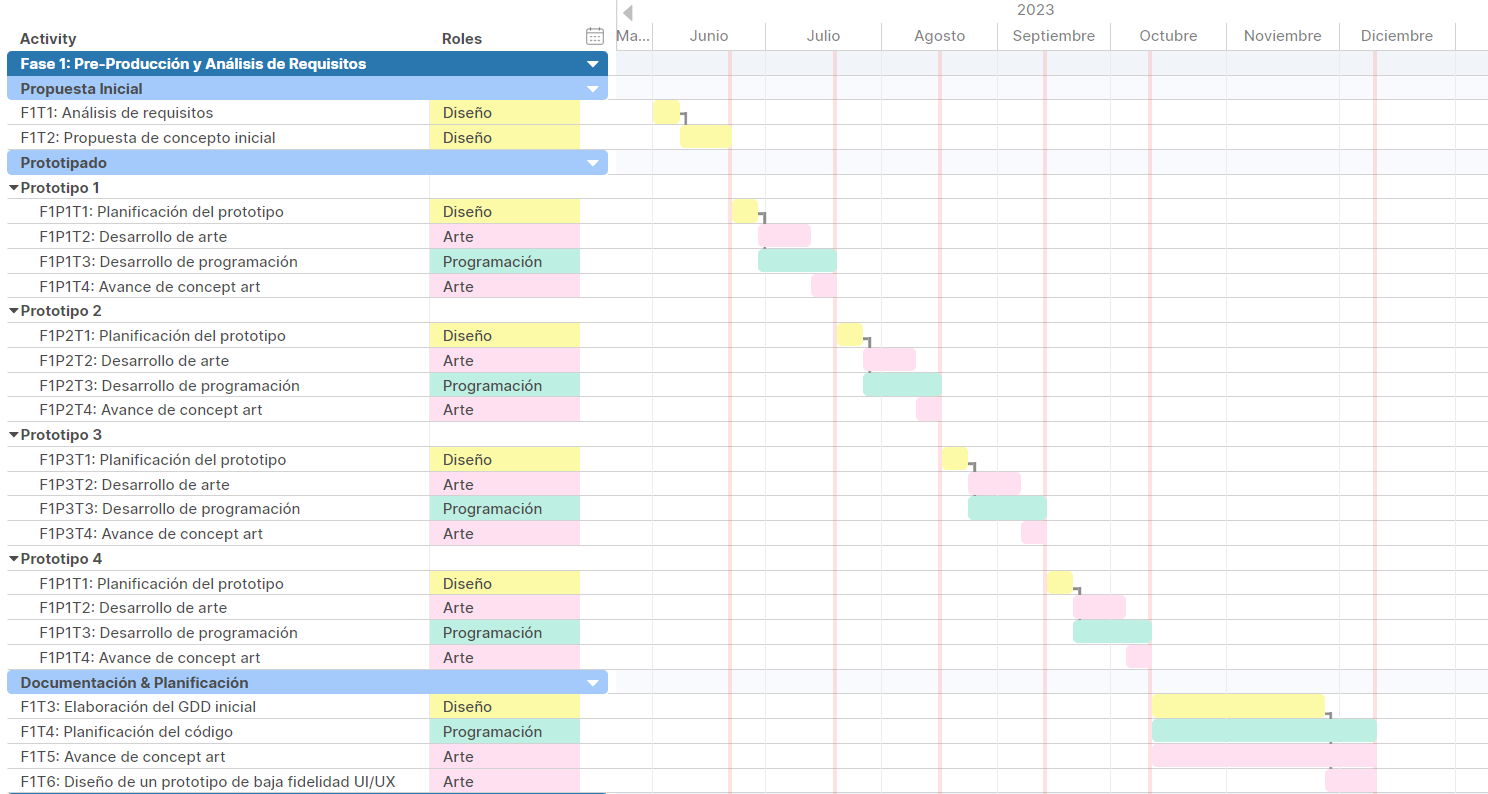
\includegraphics[width=350px,clip=true]{gantt1.png}
  \caption{Diagrama de Gantt de la fase 1 de producción}
  \label{fig:fase1gantt}
\end{figure}

\subsection{Fase 2: Producción (Enero 2025 - Mayo 2025)}

Esta fase se detalla en el diagrama de la figura \ref{fig:fase2gantt}, donde se puede observar la planificación para el desarrollo de una librería 
'feature complete' pero sin pulido, ni el contenido final.

\subsubsection{Primer Hito (17 de marzo)}

\begin{compactitem}
\item F2P1T1: Implementación final de sistemas prototipados, diálogo, mazmorras, experiencia, guardado, sacudida de cámara y audio. (21 de enero - 10 de marzo)
\item F2P1T2: Implementación prototipo del sistema de animaciones de texto y componentes de movimiento (11 de marzo - 17 de marzo)
\end{compactitem}

\subsubsection{Segundo Hito (21 de abril)}

\begin{compactitem}
\item F2P2T1: Implementación final del sistema de animaciones de texto y componentes de movimiento (18 de marzo - 11 de abril)
\item F2P2T2: Implementación inicial de componentes Floater, LookAtCamera, LaunchRigidbody, vida e interacción (11 de abril - 21 de abril)
\end{compactitem}

\subsubsection{Tercer Hito (26 de mayo)}

\begin{compactitem}
\item F2P3T1: Implementación final de componentes Floater, LookAtCamera, LaunchRigidbody, vida e interacción. (22 de abril - 26 de abril)
\item F2P3T2: Implementación de componentes de debug (27 de abril - 19 de mayo)
\item F2P3T3: Pulido y testing de herramientas (20 de mayo - 26 de mayo)
\end{compactitem}

\begin{figure}[H]
  \centering
	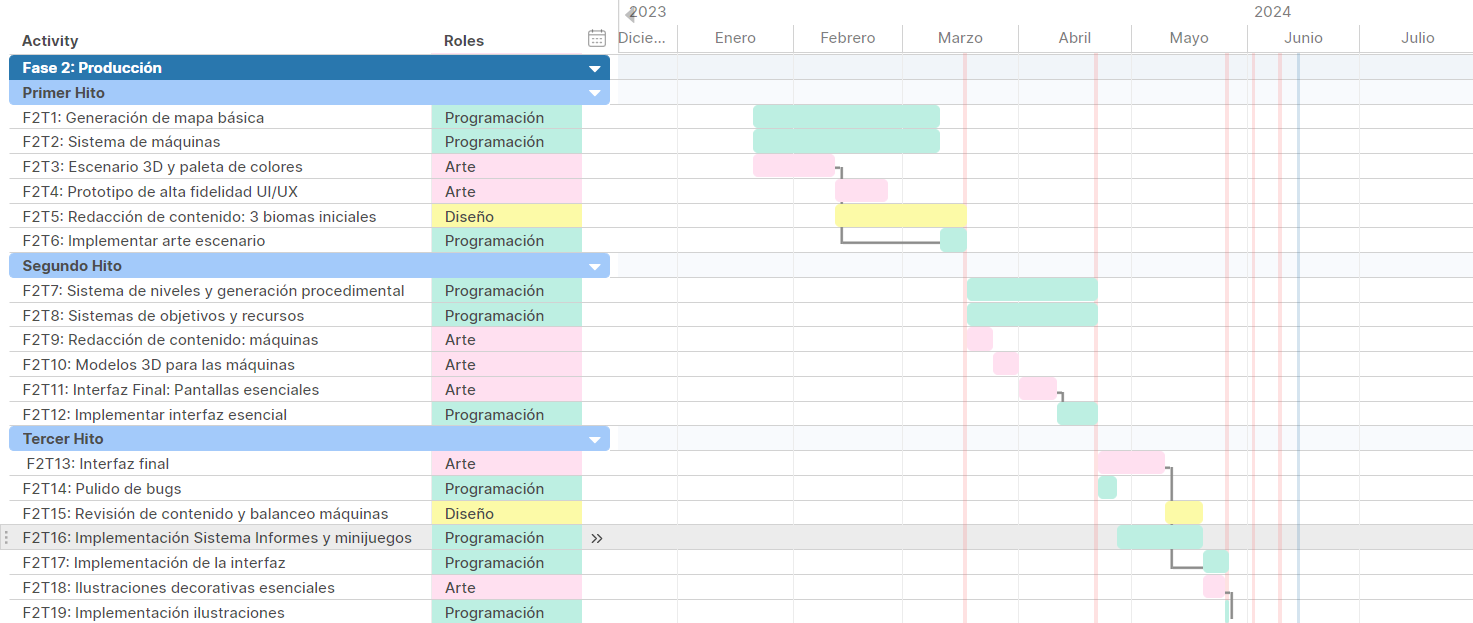
\includegraphics[width=350px,clip=true]{gantt2.png}
  \caption{Diagrama de Gantt de la fase 2 de producción}
  \label{fig:fase2gantt}
\end{figure}

\subsection{Fase 3: Polish, Desarrollo de Niveles de Prueba, Documentación y Validación (Junio 2025)}

En el diagrama de la figura \ref{fig:fase3gantt} se puede ver el desarrollo de la fase final, donde se ha terminado de pulir y completar la librería, 
así como se ha desarrollado la documentación y niveles de prueba para ayudar a los usuarios, culminando así con la propia validación con dichos usuarios.

\subsubsection{Primer Hito (2 de junio)}

\begin{compactitem}
\item F3P1T1: Pulido de bugs visuales en sistema de diálogo, desarrollo de animaciones de texto adicionales. (27 de mayo - 2 de junio)
\item F3P1T2: Redacción de documentación y niveles de prueba (27 de mayo - 2 de junio)
\end{compactitem}

\subsubsection{Segundo Hito (9 de junio)}

\begin{compactitem}
\item F3P2T1: Validación con agentes independientes (2 de junio - 9 de junio)
\end{compactitem}

\subsubsection{Tercer Hito (13 de junio)}

\begin{compactitem}
  \item F3P3T1: Procesado de los resultados de las encuestas de validación y últimos retoques (10 de junio - 13 de junio)
\end{compactitem}

\begin{figure}[H]
  \centering
	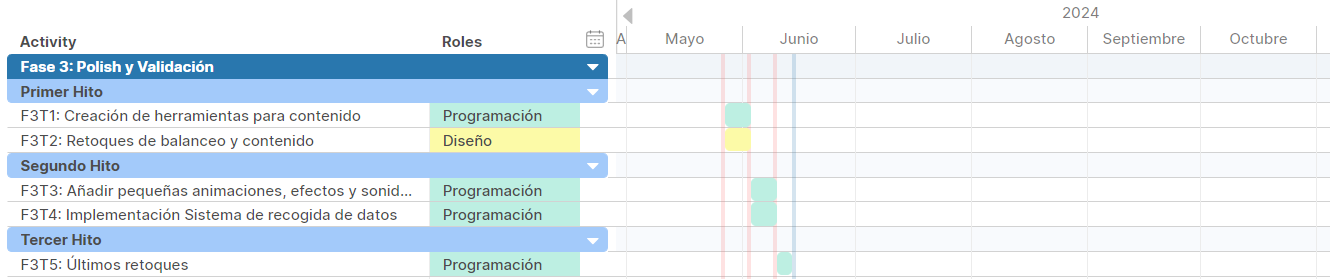
\includegraphics[width=350px,clip=true]{gantt3.png}
  \caption{Diagrama de Gantt de la fase 3 de producción}
  \label{fig:fase3gantt}
\end{figure}

Lo más destacable tras haber seguido esta metodología es haber hecho un esfuerzo inicial en prototipado y un firme análisis de requisitos 
previo, esto ha permitido tener una base muy sólida sobre la que trabajar, y tener muy claro en todo momento el objetivo, lo cual ha resultado indispensable 
para poder lograr la consecución de los objetivos a la larga.

% \afterpage{\blankpage} % puede generar problema en índice de contenidos
% \newpage

% Capítulo 2
\chapter{Estado del Arte}
\label{sec:estadodelarte}

\section{Herramientas alternativas a DUJAL}
Previo al desarrollo del paquete, se hizo una investigación para buscar referencias acerca de otras herramientas similares a los componentes,
 tanto como para buscar inspiración, como para encontrar posibles limitaciones que paliar. A continuación se discute el estado del arte de algunos de los componentes más relevantes del paquete de herramientas.

\subsection{Sacudida de Cámara}
Las herramientas de sacudida de cámara o 'Screen Shake' no son demasiado populares o comunes en la Unity Asset Store\cite{unityAssetStore}, quizás se deba a la gran cantidad de tutoriales acerca del tema disponibles en 
todo internet. Sin embargo, tal y como evidencia un pequeño estudio desarrollado por Jump Trajectory: 'Screenshake that doesn’t suck'\cite{Screenshake}, la técnica utilizada por la mayoría de estos tutoriales es deficiente
y trae consigo serios problemas cuando se trabaja en espacios tridimensionales. El pricipal problema de estas es que al aplicar una traslación a una cámara en este tipo de espacios se puede provocar que dicha cámara acabe dentro 
de la geometría el nivel. Esto provoca un fenómeno conocido como 'clipping' (Figura \ref{fig:clipping}). Este problema se puede ver muy claramente en uno de los primeros resultados relacionados con la sacudida de cámara en la Unity Asset 
Store\cite{unityAssetStore}, el paquete de Camera Shake FX\cite{ShakeFX}. Otro de los paquetes más populares de sacudida de cámara es Camera Shake Pro\cite{ShakePro}, que pese a ser mucho más completo y no tener los problemas 
que presenta Jump Trajectory en su estudio, tampoco incluye una forma sencilla de definir curvas o líneas de animación que controlen la intensidad de la sacudidas. La implementación de DUJAL pretende incluir las observaciones 
de Jump Trajectory en su estudio, además de las funcionalidades de calidad de vida de Camera Shake Pro\cite{ShakePro} tales como traer prefabs que permitan tener al sistema funcionando en menos de dos minutos, tener 
efectos predefinidos que prescindan al usuario de tener que crear unos nuevos, o que la llamada al componente de sacudida sea una función estática y global para mayor facilidad de uso en el código. Además de incluir algunas
funcionalidades propias, como las previamente mencionadas curvas de animación que permitan crear infinitas sacudidas únicas de forma visual e intuitiva.

\begin{figure}[H]
    \centering
    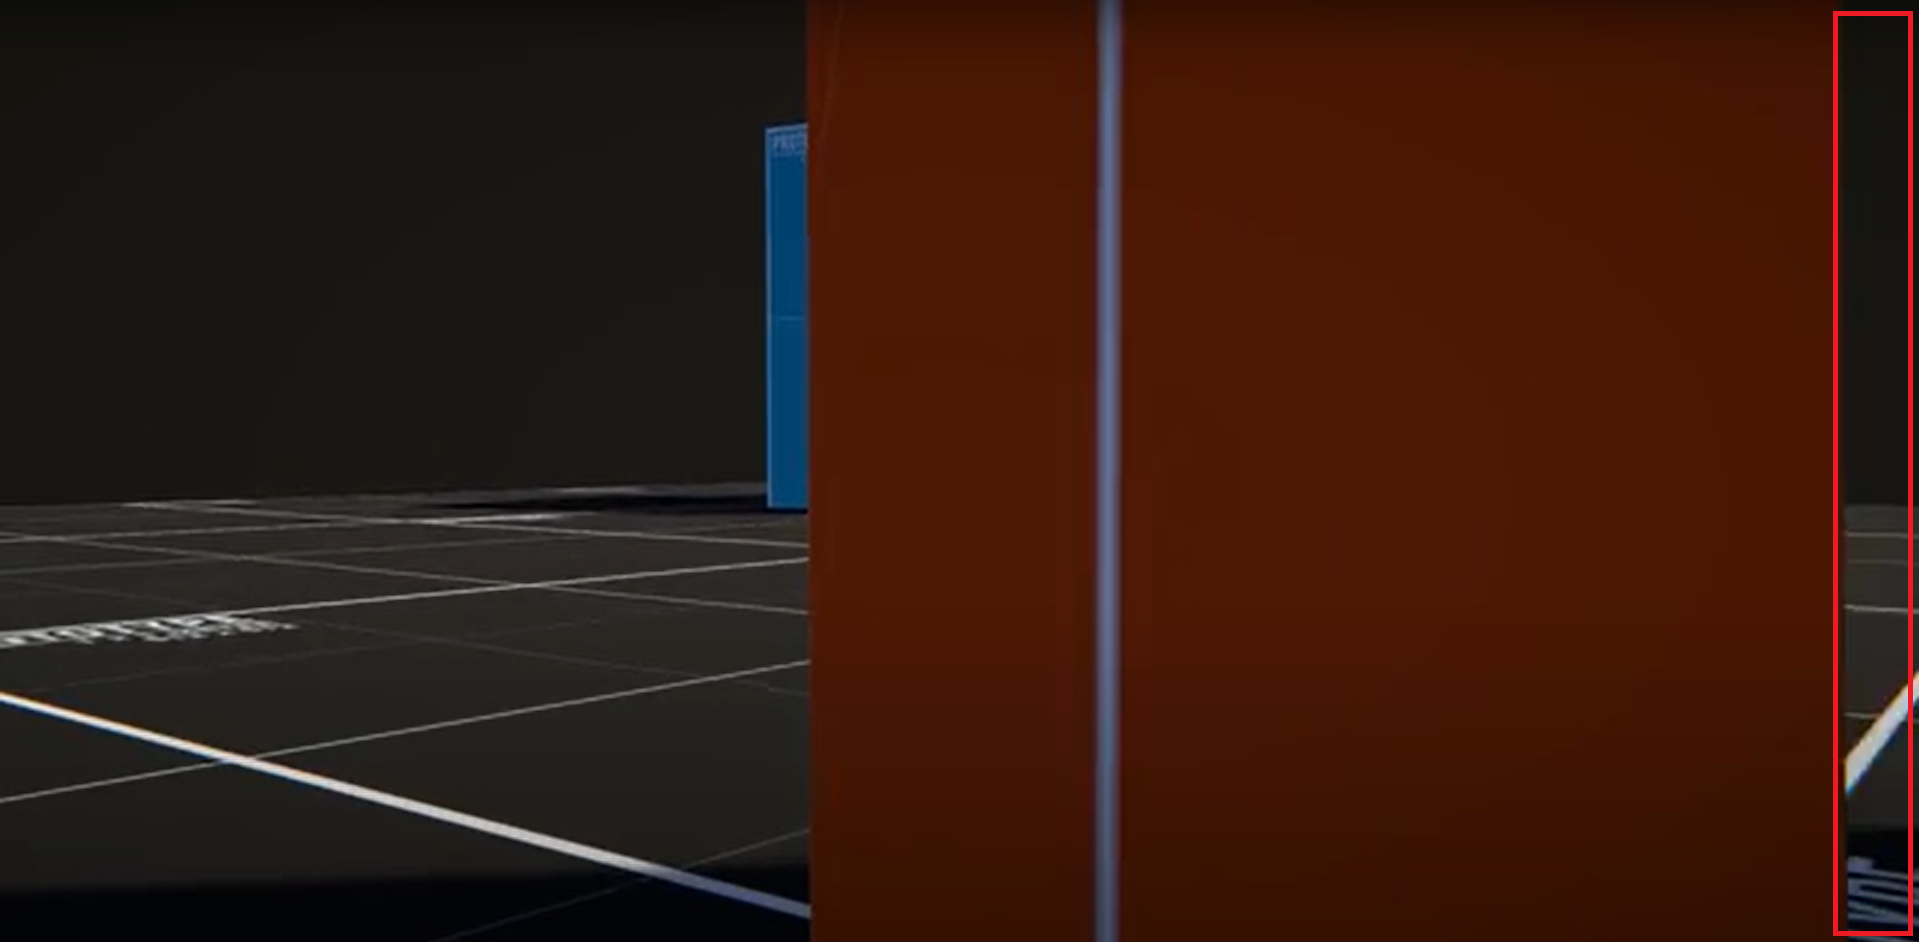
\includegraphics[width=350px,clip=true]{clipping.png}
    \caption{Representación del 'Cipping'}
    \label{fig:clipping}
\end{figure}

\subsection{Herramientas de Diálogos}
Con respecto a las herramientas de generación de diálogos hay una herramienta que es claramente el estándar, Dialogue System for Unity\cite{DialogueSystemUnity}, esta herramienta ha sido utilizada por algunos de los 
juegos más famosos de los últimos años, como Disco Elysium\cite{DiscoElysium} (Figura \ref{fig:discoelysium}) o 1000XRESIST\cite{1000xResist} (FIgura \ref{fig:1000xResist}). Es increíblemente completa dado que trae 
decenas de pequeñas herramientas para facilitar la implementación de diálogos en un juego. Permite exportar, guardar, modificar y localizar miles de textos de forma ligera y portable. El componente del Sistema de
 Diálogos de este proyecto se ha desarrollado usando esta herrameinta como referencia, con la diferencia de, en lugar de priorizar incluir los cientos de funcionalidades que forman parte de esta, priorizar la 
 facilidad de uso y la sencillez de la herramienta dado que ese es uno de los objetivos principales del proyecto. Dialogue System for Unity, aparte de ser menos accesible por ser de pago, requiere una inversión de 
 tiempo considerable para aprender a usarse, por otro lado, el componente creado para el proyecto se compone de una herramienta que permite traducir un esquema basado en grafos a un 'prefab' que se puede arrastrar 
 directamente a la escena de Unity y permite reproducir dicho diálogo sin necesidad de programar ni una sola línea de código.

\begin{figure}[H]
    \centering
    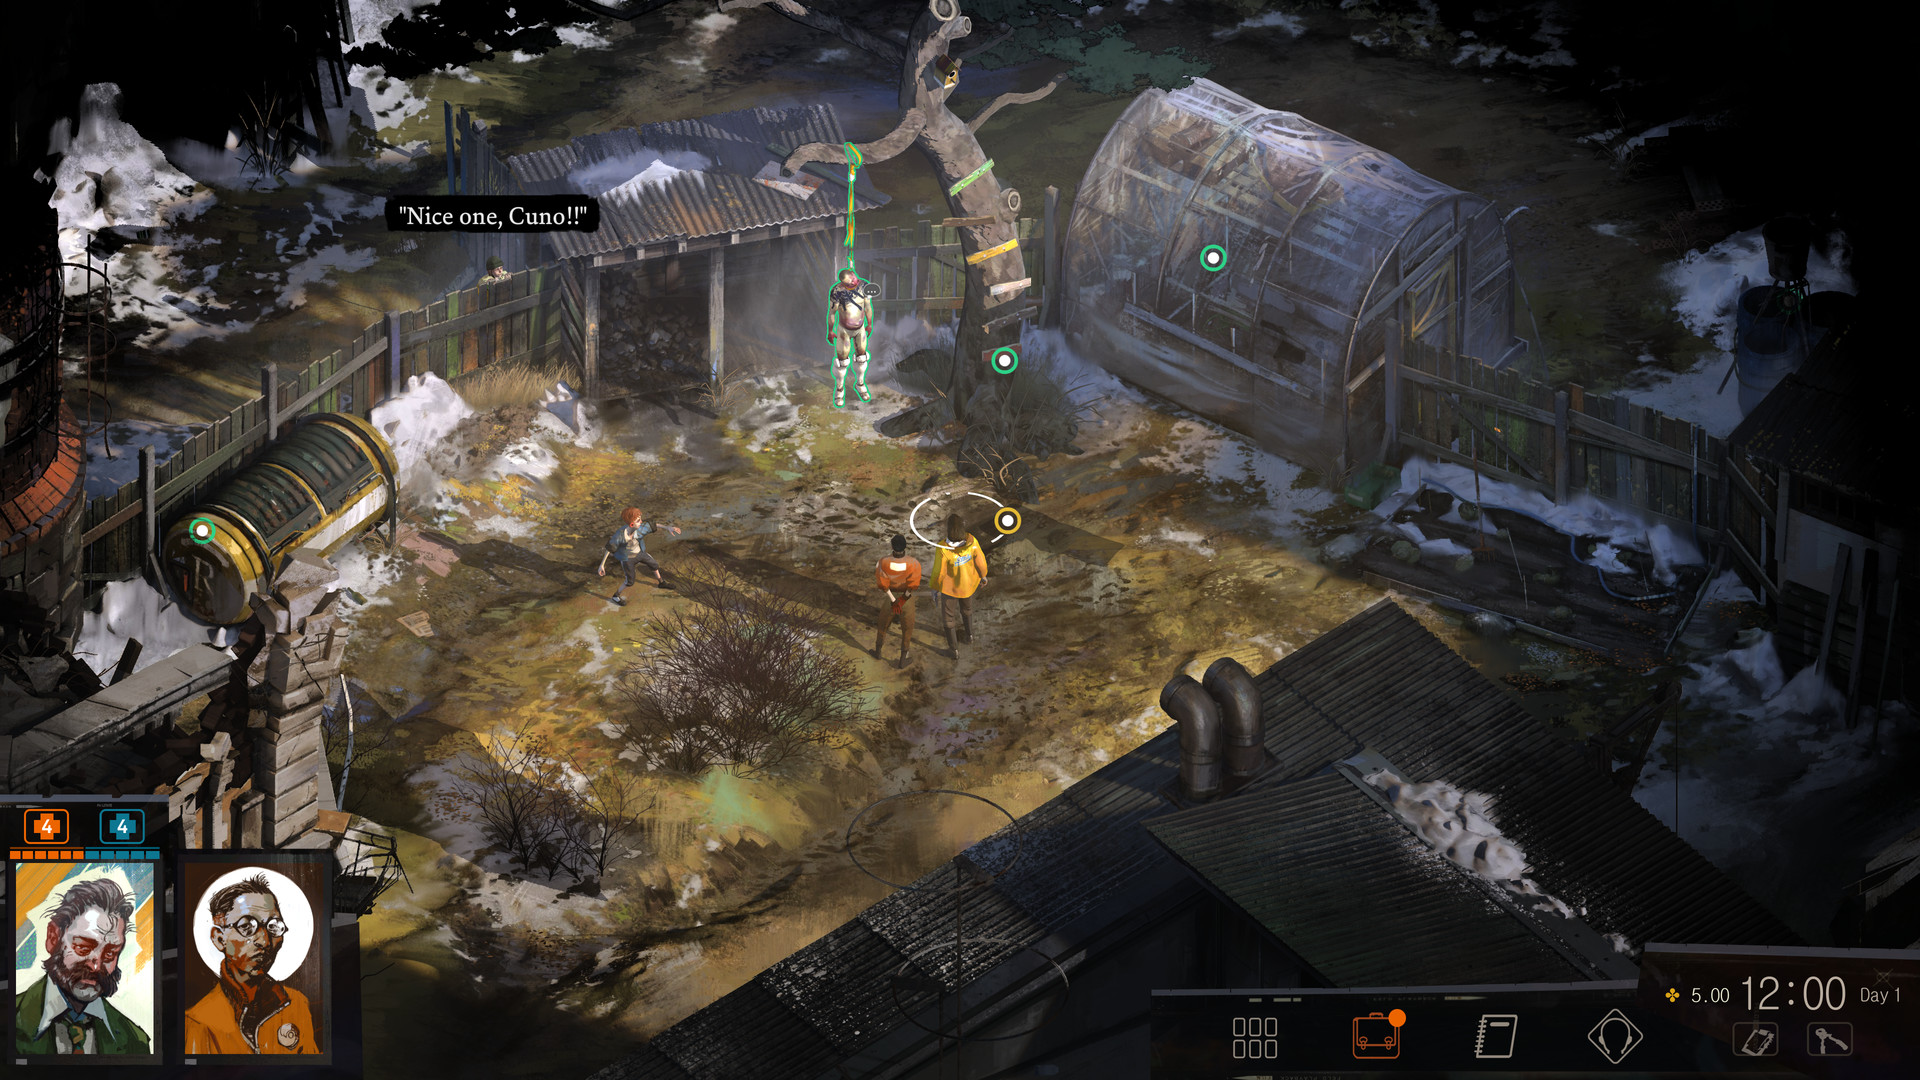
\includegraphics[width=350px,clip=true]{disco_elysium.png}
    \caption{Disco Elysium}
    \label{fig:discoelysium}
\end{figure}

\begin{figure}[H]
  \centering
  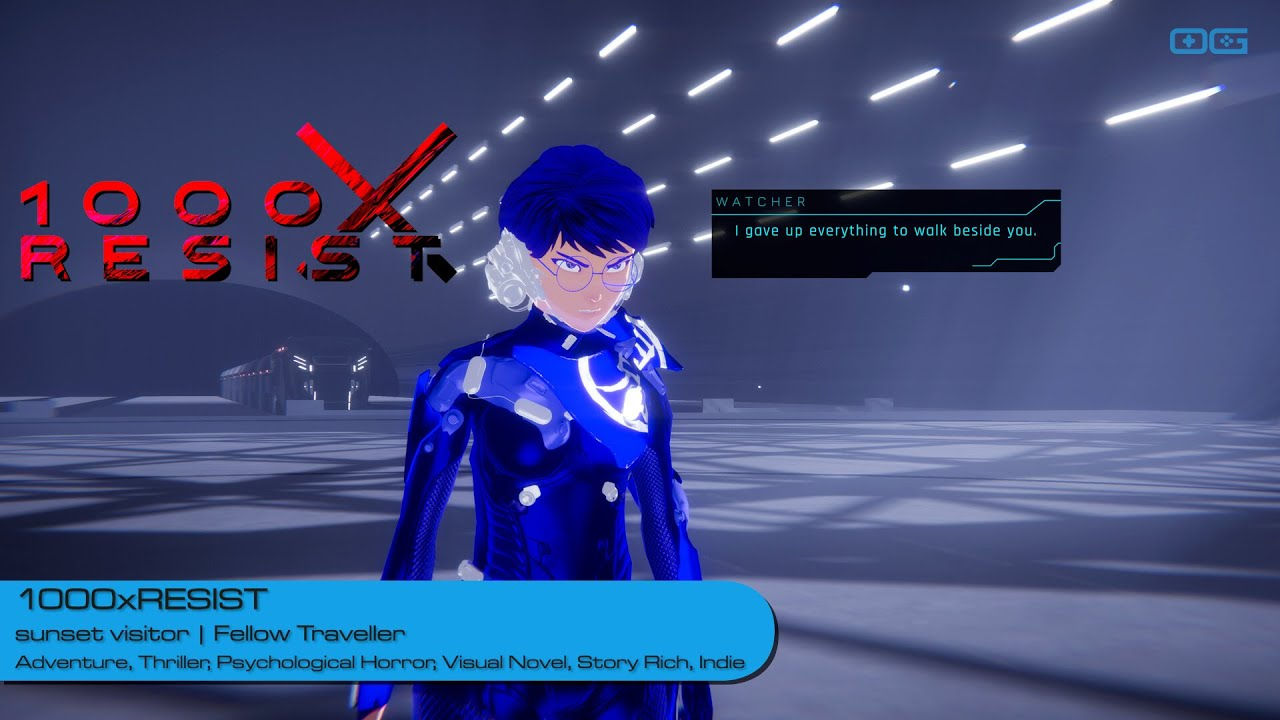
\includegraphics[width=350px,clip=true]{100xresist.png}
  \caption{1000xRESIST}
  \label{fig:1000xResist}
\end{figure}

 \subsection{Herramientas de Animación de Texto}
En lo referente a las animaciones de texto, hay una única herramienta que se corona como la más completa y profesional de todas, Text Animator\cite{TextAnimator}, desarrollada por febucci y utilizada en proyectos
 de gran envergadura, como Dredge (Figura \ref{fig:dredge}) o Cult of the Lamb (Figura \ref{fig:clamb}). Esta herramient permite añadir efectos a componentes Text Mesh Pro utilizando etiquetas similares a las de 
 Rich Text Format (usando signos de mayor y menor que). En estas se indica el tipo del efecto (fade Texto de Ejemplo /fade), también admite modicadores de tiempo, intensidad o delay. La implementación de DUJAL es muy parecida, incluso utilizando 
 un formato muy similar a la hora de incluir efectos en el texto. La principal diferencia es que la estructura del procesado de efectos permite añadir, de forma sencilla y con una sintaxis muy parecida al scripting, 
 nuevos efectos a la librería de efectos del proyecto. Además, al ser un proyecto open source, es teóricamente sencillo publicar el código que permita añadir nuevos efectos a la librería.

\begin{figure}[H]
  \centering
  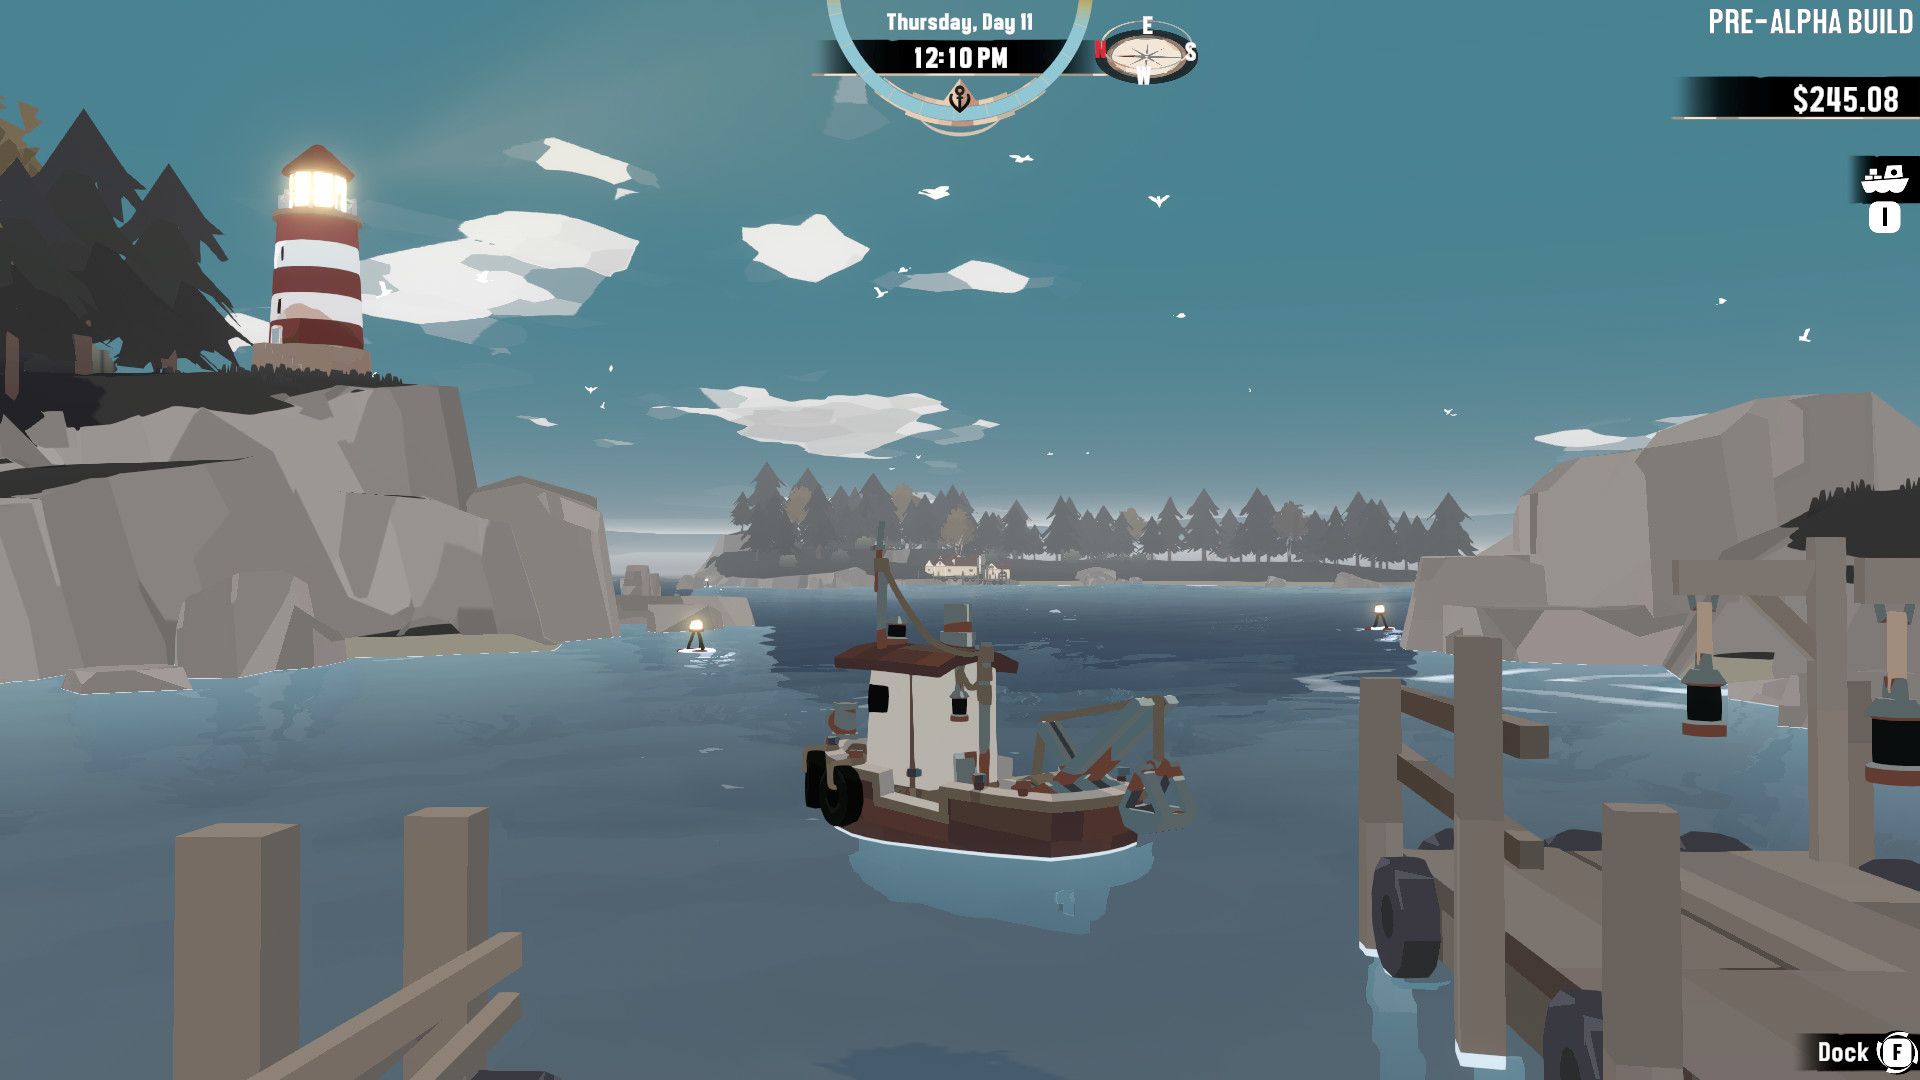
\includegraphics[width=350px,clip=true]{dredge.png}
  \caption{Dredge}
  \label{fig:dredge}
\end{figure}

\begin{figure}[H]
    \centering
    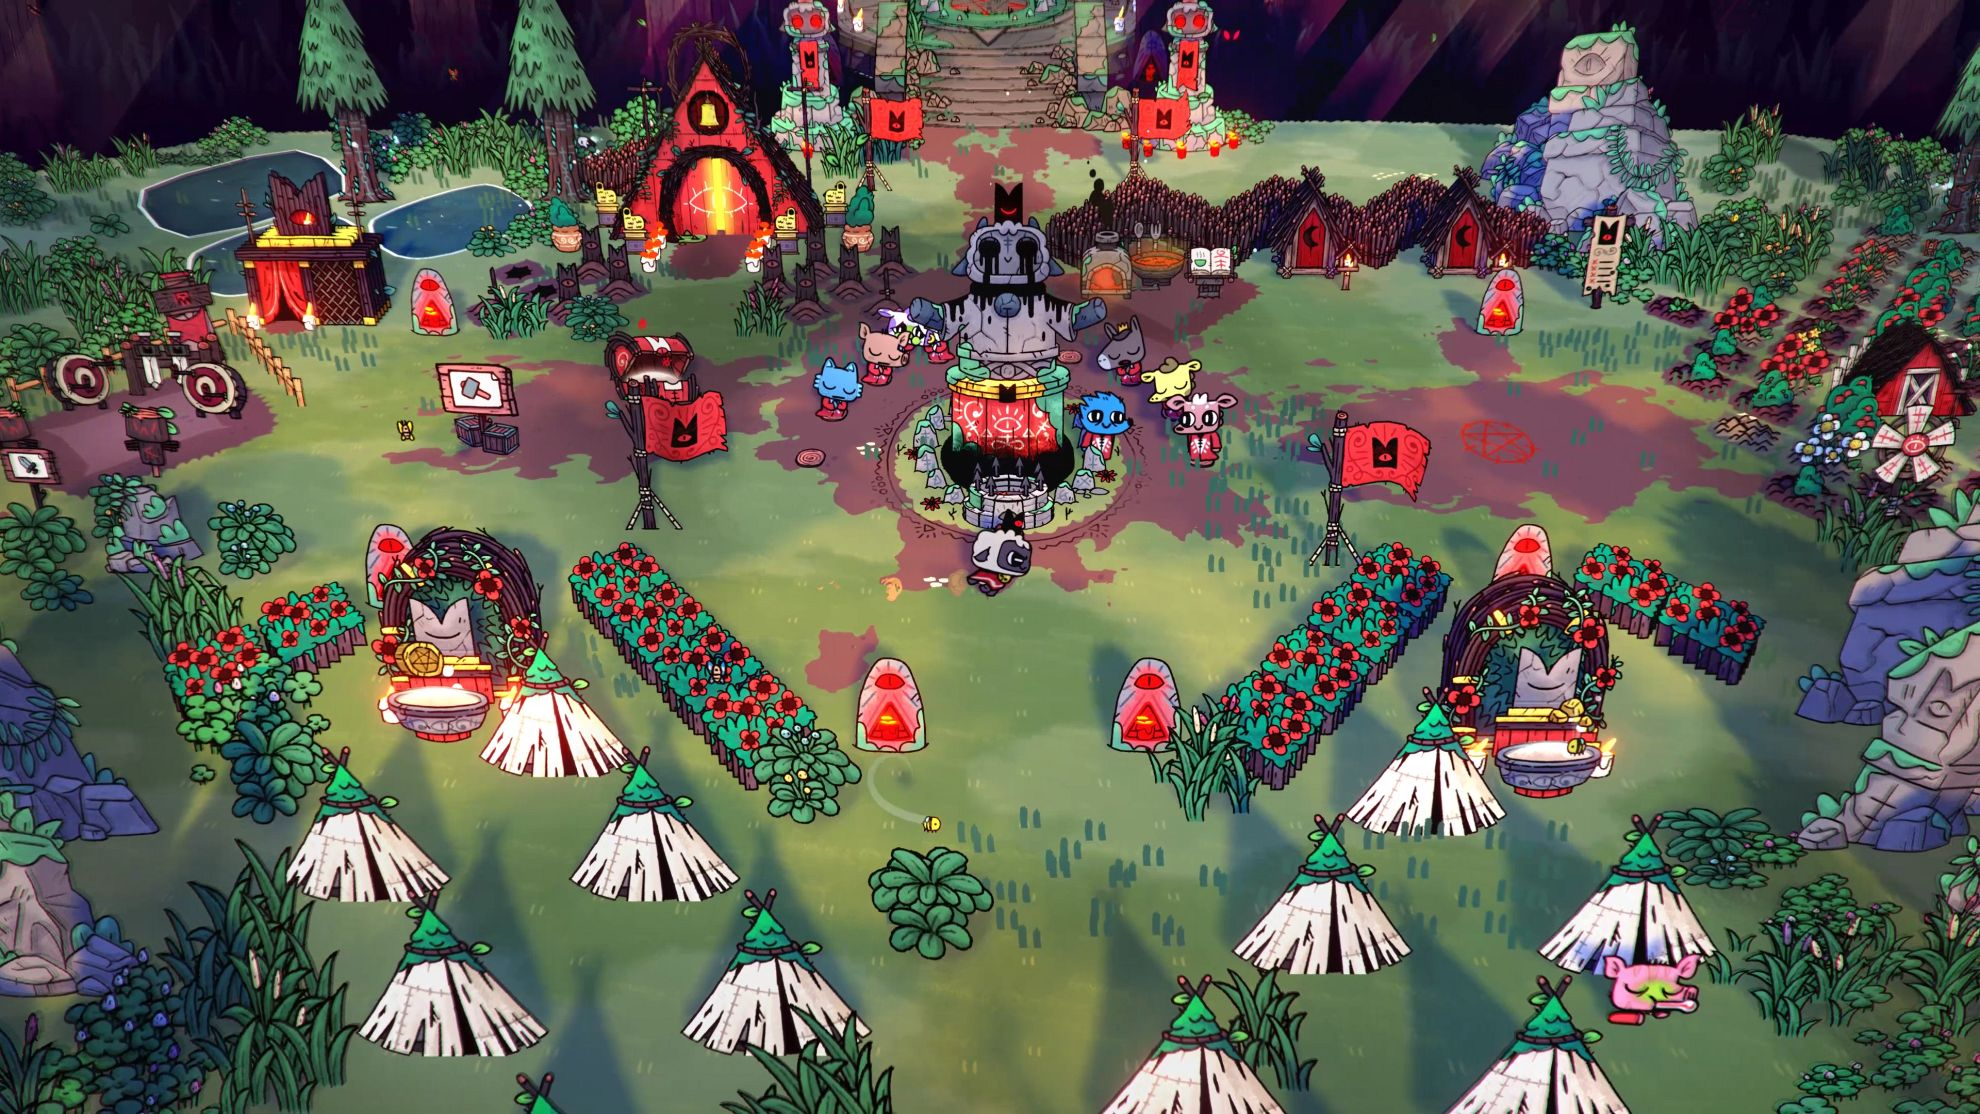
\includegraphics[width=350px,clip=true]{cult_of_the_lamb.png}
    \caption{Cult of the Lamb}
    \label{fig:clamb}
\end{figure}

\subsection{Herramientas de Movimiento de Personajes}
En la Unity Asset Store\cite{unityAssetStore} es muy común encontrar paquetes que incluyan controladores de personajes de distintos tipos. Lo normal es que permitan unicamente un tipo de movimiento concreto ajustado
 a un tipo de cámara, si el espacio es 2D o 3D o si el movimiento está regido por físicas o no. En algunos casos, como el de Easy Character Movement 2\cite{ECM2} si que se incluye un entorno más genérico que permite,
 con trabajo adicional, contar con algunas (o todas) las combinaciones de los factores mencionados anteriormente. En el caso de DUJAL, sin embargo, se quieren implementar todas las combinaciones posibles de dichos 
 factores de antemano con el objetivo de tener el completo abanico de posibilidades de movimiento sin necesidad de trabajo adicional por parte del usuario, además de expandir las funcionalidades que se suelen 
 definir estándar, como por ejemplo la posibilidad del 'Wall Running'\cite{wallRun}, 'Wall Jumping'\cite{wallJump} o 'Dashing'\cite{dash}.

\subsection{Herramientas de Generación de Mazmorras}
Respecto a las herramientas de generación de mazmorras al igual que ocurre con las de sacudida de cámara, no parece que haya demasiadas opciones. La más relevante sería Procedural Dungeon 
Generator\cite{ProceduralDunGen}, que permite la generación de mazmorras del estilo Dungeon Crawler o Roguelike de forma procedimental dados unos parámetros de entrada (Como tamaño, numero de salas, tipos de sala etc...).
Del mismo modo, el Generador de Mazmorras de DUJAL permite algo muy similar, con el añadido de permitir además generar laberintos usando un algoritmo muy similar.

\subsection{Resumen del Estado del Arte}
Como queda patente en esta sección, en lo referente a herramientas auxiliares al desarrollo de videojuegos hay una infinidad de opciones que usar, y aunque puedan haber opciones mejores, peores, más caras o más baratas,
es muy difícil que una en concreto se ajuste a un caso de uso particular, las opciones se reducen siempre a invertir un tiempo significativo en adaptar el juego que se esté desarrollando a una ya existente, o por el contrario, 
crear la herramienta de cero. El código del que se compone DUJAL pretende ser fácilmente escalable para poder ajustar la herramienta al juego, en lugar de al revés, para intentar lidiar con ese roce que tiende a ocurrir al 
buscar herramientas externas al motor.

% Capítulo 3
\chapter{Descripción Informática}
\label{sec:descripcionInformatica}

\section{Requisitos}

En esta sección se abordarán los requisitos planteados en el paquete, tanto los iniciales como los que se han ido planteando a lo largo del desarrollo ya sean funcionales o no funcionales. 

\subsection{Requisitos Funcionales}
\begin{itemize}
    \item RF1. Como usuario puedo utilizar el editor de diálogos para crear cajas y conexiones que representen conversaciones.
    \item RF2. Como usuario puedo exportar los diálogos de forma que sean legibles por el código del juego.
    \item RF3. Como usuario puedo reproducir los diálogos en el juego.
    \item RF4. Como usuario puedo añadir etiquetas al texto para reproducir animaciones del texto.
    \item RF5. Como usuario puedo utilizar el sistema de guardado para que mi juego tenga datos persistentes.
    \item RF6. Como usuario puedo usar el sistema de carga para cargar y descargar recursos.
    \item RF7. Como usuario puedo manejar los sonidos que aparecen en mi juego a través del sistema de sonido.
    \item RF8. Como usuario puedo añadir un sistema de niveles a mi juego mediante el sistema de experiencia.
    \item RF9. Como usuario puedo insertar un personaje jugable con cámara en cualquier perspectiva.
    \item RF10. Como usuario puedo insertar un personaje jugable con movimiento basado en físicas o discreto.
    \item RF11. Como usuario puedo insertar un personaje jugable ya sea en 2D o 3D.
    \item RF12. Como usuario puedo depurar las herramientas del paquete.
    \item RF13. Como usuario puedo generar una mazmorra o un laberinto usando el generador de mazmorras.
    \item RF14. Como usuario puedo utilizar algoritmos para encontrar el camino mínimo para salir de un laberinto o llegar a la hora de una mazmorra.
    \item RF15. Como usuario puedo modificar el tamaño y posición de una mazmorra.
    \item RF16. Como usuario puedo hacer que un objeto flote y rote.
    \item RF17. Como usuario puedo añadir interacciones a mi juego.
    \item RF18. Como usuario puedo añadir vida, daño y muerte a mi juego.
    \item RF19. Como usuario puedo añadir lanzar un objeto que utilice físicas en cualquier dirección.
    \item RF20. Como usuario puedo hacer que un objeto siempre mire a cámara.
    \item RF21. Como usuario puedo utilizar curvas de animación para sacudir la cámara en 2D y 3D, para cámaras de Unity y Cinemachine.
\end{itemize}

\subsection{Requisitos No Funcionales}

\begin{itemize}
    \item RNF1. Los módulos del paquete deben ser escalables.
    \item RNF2. Los módulos del paquete deben estar documentados.
    \item RNF3. El código del paquete debe ser legible y estar bien estructurado.
    \item RNF4. El paquete debe ser usable y recibir buenos resultados en las encestas de satisfacción.
\end{itemize}

\section{Herramientas y Tecnologías}

\subsection{C\# \& Unity}

Se ha utilizado Unity\cite{unity} como motor para el que está diseñado el paquete y C\#\cite{csharp} como lenguaje de programación, se ha elegido este motor dado que era el motor público más utilizado por estudiantes y equipos pequeños y medianos.

\subsection{Visual Studio}

Visual Studio\cite{visualstudio} es un IDE y editor de código para C++ y .Net y C\#, es el editor de código por defecto de Unity y el que se ha utilizado por defecto para el desarrollo del proyecto. 

\subsection{Git \& Github}

Github\cite{github} es un entorno de desarrollo colaborativo y control de versiones web basado en la tecnología Git. Para mantener el proyecto y poder trabajar en el desde distintos equipos, se ha alojado el proyecto de del paquete\cite{Repo} en él.

\subsection{UniTask}

UniTask\cite{UniTask} es una librería que ofrece una implementación de async/await sin necesidad de alocataciones de memoria basada en estructuras. Se ha aprovechado esta librería para la implementación del sistema de carga de escenas, ya que permite un funcionamiento asíncrono.

\section{Arquitectura y Análisis}
En la siguiente sección se detallan los detalles técnicos acerca del paquete, explicando los detalles de implementación de las distintas secciones, módulos y componentes.

\subsection{Sistema de Diálogos}
El sistema de diálogos está compuesto de tres subsistemas que hacen posible el renderizado de diálogo siguiendo los requisitos funcionales del proyecto. Estas tres partes son
el sistema de editor de diálogos (Figura \ref{fig:dialogueEditorExample}) (incluyendo la lógica que exporta el contenido de un diálogo a un asset que se pueda abrir), el sistema que gestiona la lógica de pintar el 
diálogo en el juego y el sistema que gestiona las animaciones del texto.

El código del editor es en parte el más complejo, ya que hace uso de la herramienta de Grafos de Unity para poder definir clases para los nodos del editor como muestra la 
Figura \ref{fig:nodos} se ha creado una clase específica por cada tipo de nodo ('Single Choice' y 'Multiple Choice'), también otra para los grupos que permiten agrupar distintos 
diálogos. También ha sido necesario crear clases para las ventanas nuevas, la del editor de diálogo, el 'GraphView' y la ventana de búsqueda.

El código de editor también se constituye de la lógica para convertir los nodos, grupos y conexiones (Figura \ref{fig:dialogueUml1}) a 'ScriptableObjects' que puedan guardarse en la memoria del dipositivo. Todo esto se gestiona mediante la clase
DialogueSystemIO (Figura \ref{fig:dialogueUml2}), que con sus funciones permite guardar, cargar y eliminar assets de tipo 'DialogueGraph'.  

\begin{figure}[H]
  \centering
    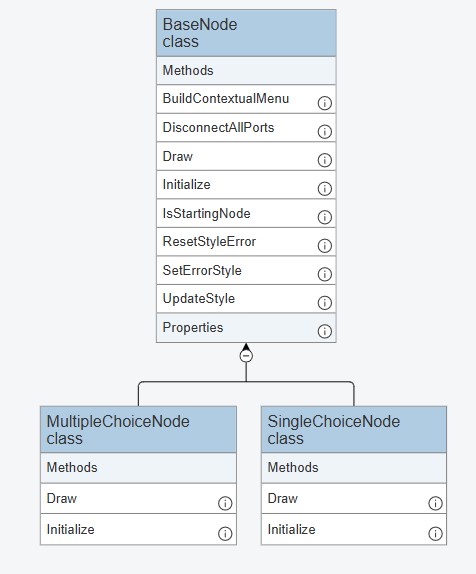
\includegraphics[width=350px,clip=true]{Node_Herencia.png}
  \caption{Diagrama de Herencia de Nodos del Sistema de Dialogo}
  \label{fig:nodos}
\end{figure}

\begin{figure}[H]
  \centering
    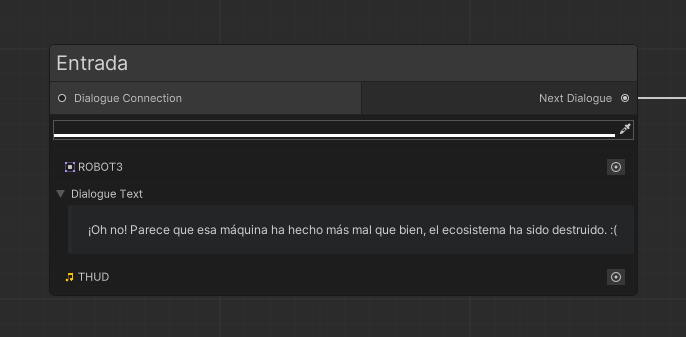
\includegraphics[width=350px,clip=true]{dialogue.png}
  \caption{Ejemplo del Editor del Sistema de Diálogo en uso}
  \label{fig:dialogueEditorExample}
\end{figure}

\begin{figure}[H]
  \centering
    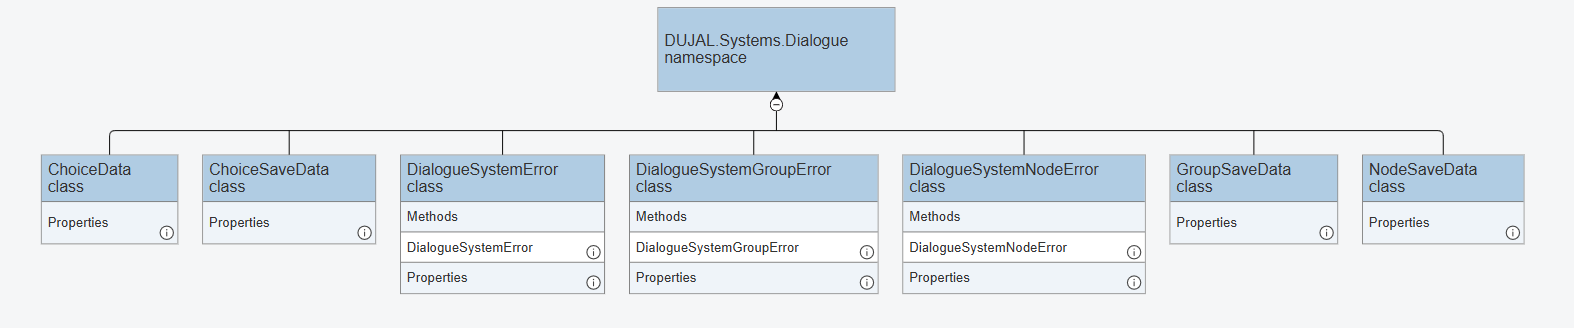
\includegraphics[width=500px,clip=true]{Dialogue_UML.png}
  \caption{Diagrama de Clases del Editor de Diálogos}
  \label{fig:dialogueUml1}
\end{figure}

\begin{figure}[H]
  \centering
    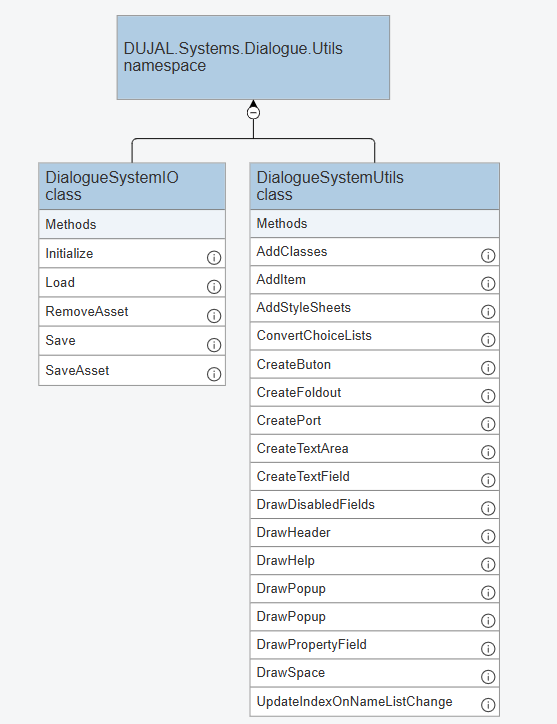
\includegraphics[width=350px,clip=true]{Dialogue_System_Utils.png}
  \caption{Diagrama de Clases Utils del Sistema de Diálogo}
  \label{fig:dialogueUml2}
\end{figure}

El sistema de dialogos de juego está compuesto por una clase de tipo Singleton que permite comenzar la reproducción del diálogo, elegir el diálogo concreto que se va a reproducir (El asset de tipo DialogueGraph que 
se quiere usar y el diálogo en concreto por el que se quiere comenzar la conversación) y configurar la reproducción de diálogo seleccionando cosas como la velocidad del texto, si se reproduce automáticamente, si se 
muesta todo el texto instantáneamente o se muestra en estilo 'Typewriter' etc. La gestión lógica de los diálogos se hace mediante un sencillo sistema de input en la que, mediante teclas, botones o el ratón, el el usuario
puede indicar que desea pasar al siguiente diálogo o elegir una opción concreta en el caso de que sea un nodo que permite ramificaciones. En lógica se selecciona la respuesta (0 - N) asociada al input que el usuario ha 
seleccionado. En el caso de los noos que no permiten elección múltiple, se selecciona por defecto siempre la opción cero, ya que siempre hay una sola. Esta parte del sistema también permite mostrar una imagen asociada 
a un interlocutor en concreto, o reproducir un sonido, utilizando el Sistema de Audio, asociado al interlocutor. El formato de sonido puede ser uno de tres tipos, en formato 'Gibberish' en la que se reproduce un 
sonido por cada letra mostrada en pantalla, en formato 'Unique Sound' en la que se reproduce un sonido por cada nueva caja de texto que se muestra, o en formato doblaje, en la que se reproducen las voces asociadas 
al texto mostrado. El resultado del sistema en uso se puede observar en la Figura \ref{fig:dialogueExample}.

\begin{figure}[H]
  \centering
    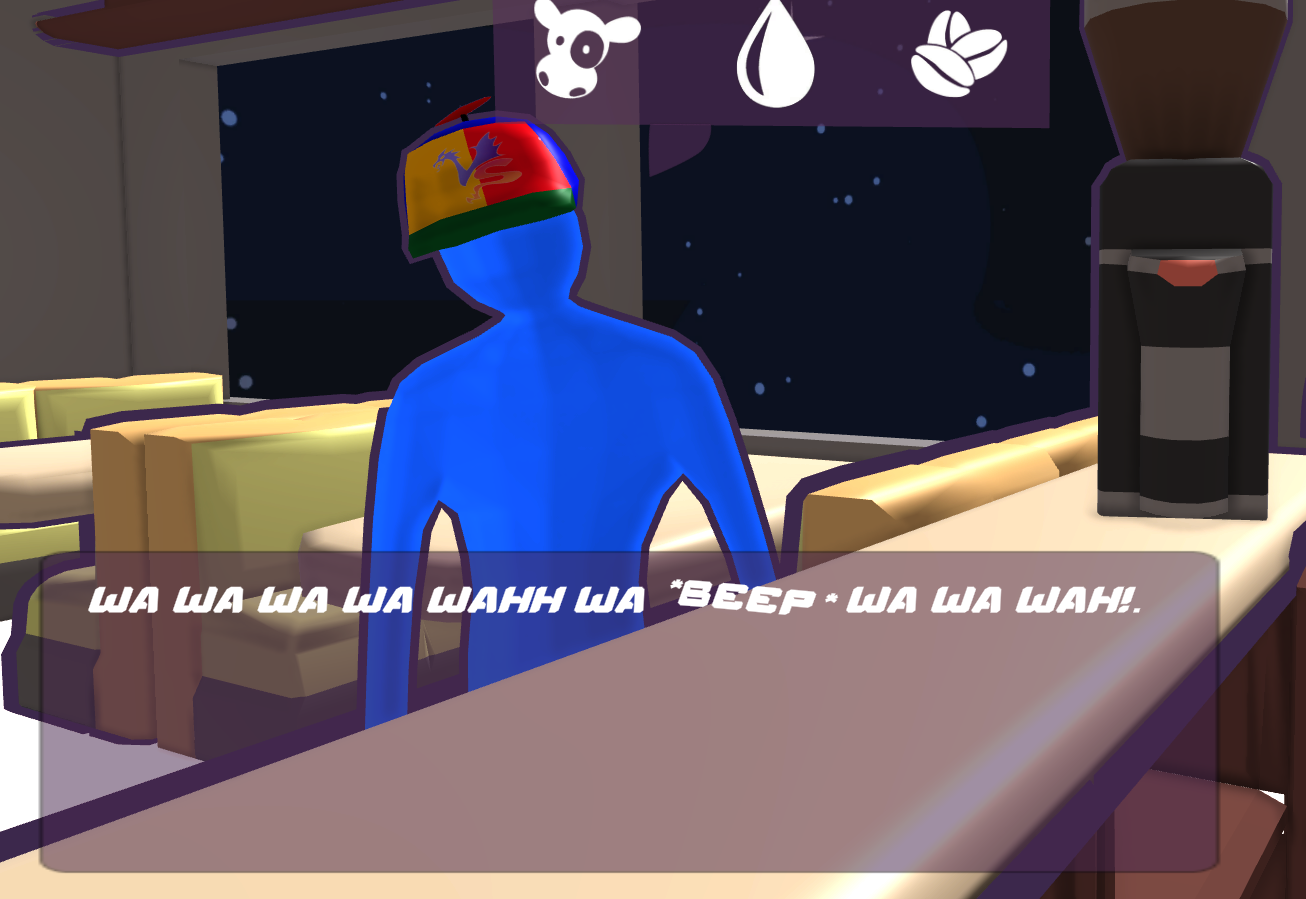
\includegraphics[width=350px,clip=true]{dialogueExample.png}
  \caption{Ejemplo del Sistema de Diálogo en uso}
  \label{fig:dialogueExample}
\end{figure}

El sistema de efectos de texto, que depende a su vez de la clase 'DialogueSystem', funciona con tags con formato '<>', el 'DialogueSystem' hace un pre-parsing del texto antes de mostrarlo al jugador para conseguir dos cosas:
en primer lugar borra las etiquetas pertinentes al 'TextEffectSystem' para que el texto se muestre como el diseñador pretendía, y, además, almacena en un mapa en el que se indican los índices del texto relevantes para aplicar 
el efecto, además de el efecto que se debe aplicar y sus modificadores. Cada efecto es gestionado por su propio tipo, dado que cada clase que hereda de TextEffect tiene sus propia implementación de 'UpdateEffect()',
tal y como se puede observar en la Figura \ref{fig:dialogueUml3}, que se utiliza mediante la Figura \ref{fig:dialogueUml4}. Lo más interesante referente al sistema de efectos de texto es que, al haber construido un
'template' la cual seguir para añadir efectos nuevos, y que el código interno y exclusivo de cada efecto es relativamente simple y pequeño, es muy sencillo escalar el sistem para añadir nuevos efectos. Una instancia
 del código de scripting mediante le cual se puede añadir un efecto nuevo se puede encontrar en el Código \ref{alg:wobbleAnimation}.

\begin{figure}[H]
  \centering
    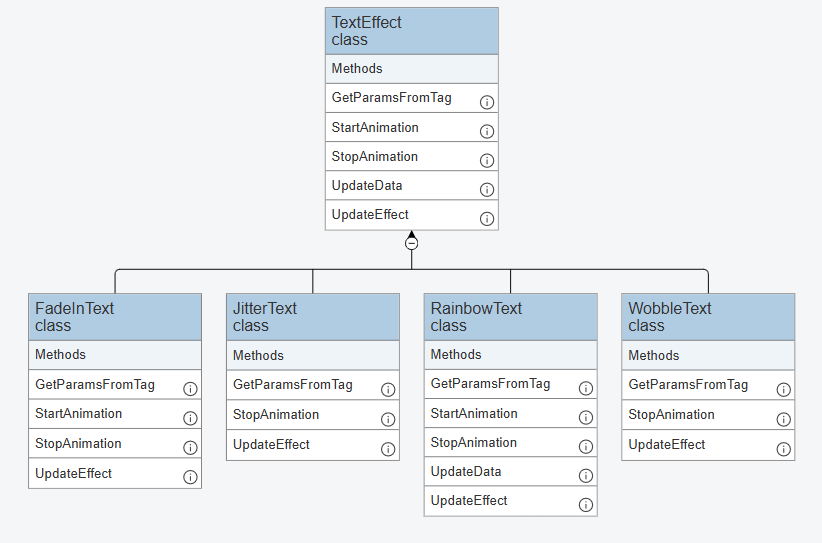
\includegraphics[width=350px,clip=true]{Text_Effects.png}
  \caption{Diagrama de Clases de Animaciones de Texto}
  \label{fig:dialogueUml3}
\end{figure}


\begin{figure}[H]
  \centering
    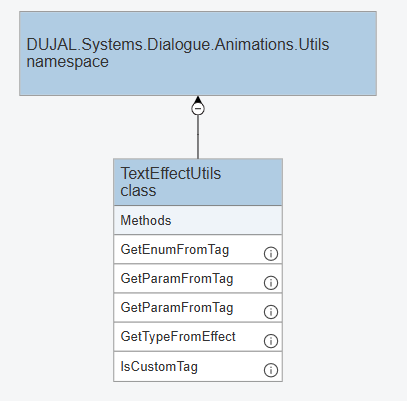
\includegraphics[width=350px,clip=true]{Text_Effect_Utils.png}
  \caption{Diagrama de Clases Utils del las Animaciones de Texto}
  \label{fig:dialogueUml4}
\end{figure}

\begin{mypython}[caption={Ejemplo de código utilizado para definir la animación de 'Wobble' en el texto.},label={alg:wobbleAnimation}]
    foreach (EffectInstance effect in effects) 
    {
        for (int i = effect.TextStartIdx; i < effect.GetTextEndIndex(); ++i)
        {
            var charInfo = animationHandler.TextInfo.characterInfo[i];
            if (!charInfo.isVisible)
            {
                continue;
            }
            
            var meshInfo = animationHandler.TextInfo.meshInfo[charInfo.materialReferenceIndex];
            var verts = meshInfo.vertices;
            for (int j = 0; j < 4; ++j)
            {
                int vertexIdx = charInfo.vertexIndex + j;
                float newOrigY = Mathf.Sin(Time.time * _speed[effectIdx] + verts[vertexIdx].x * 0.01f) * _amplitude[effectIdx];
                verts[vertexIdx] = verts[vertexIdx] + new Vector3(0f, newOrigY, 0f);
            }
        }
        effectIdx++;
    }
\end{mypython}

\subsection{Sistema de Experiencia}
El sistema de experiencia es un pequeño conjunto de clases que permite definir una lista de niveles de 'minLevel' a 'maxLevel' dada una función lineal, cuadrática, cúbica o 
 parabólica, este sistema permite definir callbacks para eventos de subida de nivel, aumento de experiencia y llegada al nivel máximo. El sistema gestiona automáticamente las
 subidas y el aumento de experiencia y dispone de funciones de acceso para obtener los datos actualizados en cualquier momento dado.

El sistema también cuenta con la posibilidad de crear 'ScriptableObjects' de tipo 'ExperienceMobAsset', que permiten definir la cantidad de experiencia que proporciona un evento 
 concreto, para ejemplificarlo se puede asumir que se estaría hablando de derrotar un enemigo en un juego de rol tradicional. El sistema cuenta con un manager singleton que 
 permite calcular el valor de la experiencia que daría un evento o 'Mob' concreto, además cuenta con la funcionalidad para definir distintos tipos de contextos modificadores 
 de experiencia.


\subsection{Sistema de Audio}
El sistema de audio o Audio Manager en código es una clase de tipo Singleton que permite definir una serie de 'ScriptableObjects' de tipo 'Sound'. Estos permiten a su vez que 
se les asigne un clip de audio y una serie de parámetros como si es un efecto de sonido o una canción, un modificador de volumen, de tono o si se desea que dicho sonido 
se reproduzca en bucle. La clase Audio Manager contiene a su vez un array de 'Sounds' y es capaz de reproducir, pausar, parar o reanudar cualquier sonido o canción que contenga. 
La clase tiene también la capacidad de gestionar una lista de música aleatoria de ambiente para ese tipo de juegos. El sistema tiene capacidad para separar los distintos tipos de 
sonido, música o efecto, en distintas pistas de audio con el fin de poder ajustar los dsitintos volúmenes por separado.    

\subsection{Sistema de Guardado}
El sistema de guardado está compuesto por tres clases llamadas: 'SaveDataHandler', 'SaveDataFileHandler' y 'SaveData'. 'SaveDataHandler' es una clase de tipo Singleton que 
sirve como API para gestionar las llamadas al guardado, creación de nuevos archivos de guardado u operaciones de borrado y copia de estos. El 'SaveDataFileHandler' es por 
otra parte el encargado de gestionar la conversión de datos en memoria dinámica a archivos .json almacenados en memoria estática del dispositivo. La clase 'SaveData' por últimos
es la clase en la que se almacenan los datos que se quieran guardar. El sistema soporta guardar tipos de datos alfanuméricos, listas y diccionarios de tipo 
'SerializableDictionary', dado que los diccionarios de C\# estándar no se pueden serializar a formato JSON. La implementación del 'SerializableDictionary' es muy sencilla, 
simplemente funciona como una lista de listas de tipo 'KeyValuePair', que a su vez contienen su respectiva clave y valor. Adicionalmente el sistema permite encriptar la 
partida guardada con una sencilla función de hash de XOR, de forma que no se almacene como texto en claro en el dispositivo.  

\begin{figure}[H]
  \centering
    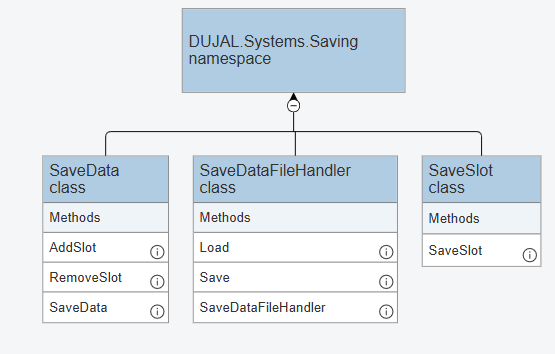
\includegraphics[width=350px,clip=true]{Saving.png}
  \caption{Diagrama de Clases del Sistema de Guardado}
  \label{fig:savinguml}
\end{figure}

\subsection{Sistema de Gestión Carga de Escenas}
El sistema de gestión de carga de escenas permite cargar de forma asíncrona y sustitutiva distntas escenas de un proyecto. El sistema automáticamente muestra una 
pantalla de carga que también esconde automáticamente una vez termina de cargar. La pantalla de carga puede mostrar opcionalmente el progreso de la carga. Añadir una nueva
 escena pasa, aparte de por añadir una nueva escena a las dependencias del proyecto en unity, por añadir un nuevo valor al enumerado de la clase 'SceneIndex'. Dicha clase 
 permite operar con 'SceneIndex' intercambiablemente como objetos, enumerados o enteros.

\subsection{Herramienta de Dibujado de Colisiones 2D}
La herramienta de dibujado de colisiones 2D (Figura \ref{fig:debug2d}), permite dibujar los colliders 2D de unity en builds empaquetadas del juego mediante el uso de
 'Line Renderers'. 

\begin{figure}[H]
  \centering
    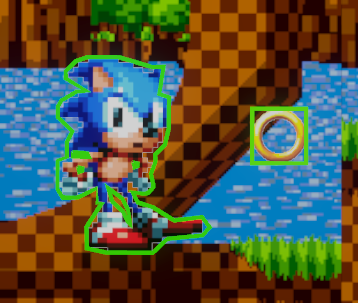
\includegraphics[width=350px,clip=true]{debug2d.png}
  \caption{Herramienta de Dibujado de Colisiones 2D en el modo 'Play' de Unity}
  \label{fig:debug2d}
\end{figure}

\begin{mypython}[caption={Algoritmo para pintar un box collider 2D.},label={alg:debugbox2d}]
    void HighlightCollider()
    {
        Vector3[] pos = new Vector3[4];
        pos[0] = transform.TransformPoint(new Vector3(_boxCol.size.x / 2.0f, _boxCol.size.y / 2.0f, 0));
        pos[1] = transform.TransformPoint(new Vector3(-_boxCol.size.x / 2.0f, _boxCol.size.y / 2.0f, 0));
        pos[2] = transform.TransformPoint(new Vector3(-_boxCol.size.x / 2.0f, -_boxCol.size.y / 2.0f, 0));
        pos[3] = transform.TransformPoint(new Vector3(_boxCol.size.x / 2.0f, -_boxCol.size.y / 2.0f, 0));
        _line.SetPositions(pos);
    }
\end{mypython}

\subsection{Herramienta de Cuadrícula}
La herramienta de cuadrícula o 'SnapToGrid' es un componente de editor que se puede añadir a cualquier objeto con un componente transform. En la configuración del componente
 se pueden definir el tamaño y altura de los elementos de la cuadrícula. Una vez añadido y configurado, el transform de dicho objeto quedará anclado a una cuadrícula como 
 célula del tamaño configurado, como se puede ver en la Figura \ref{fig:snaptogrid}.

 \begin{figure}[H]
  \centering
    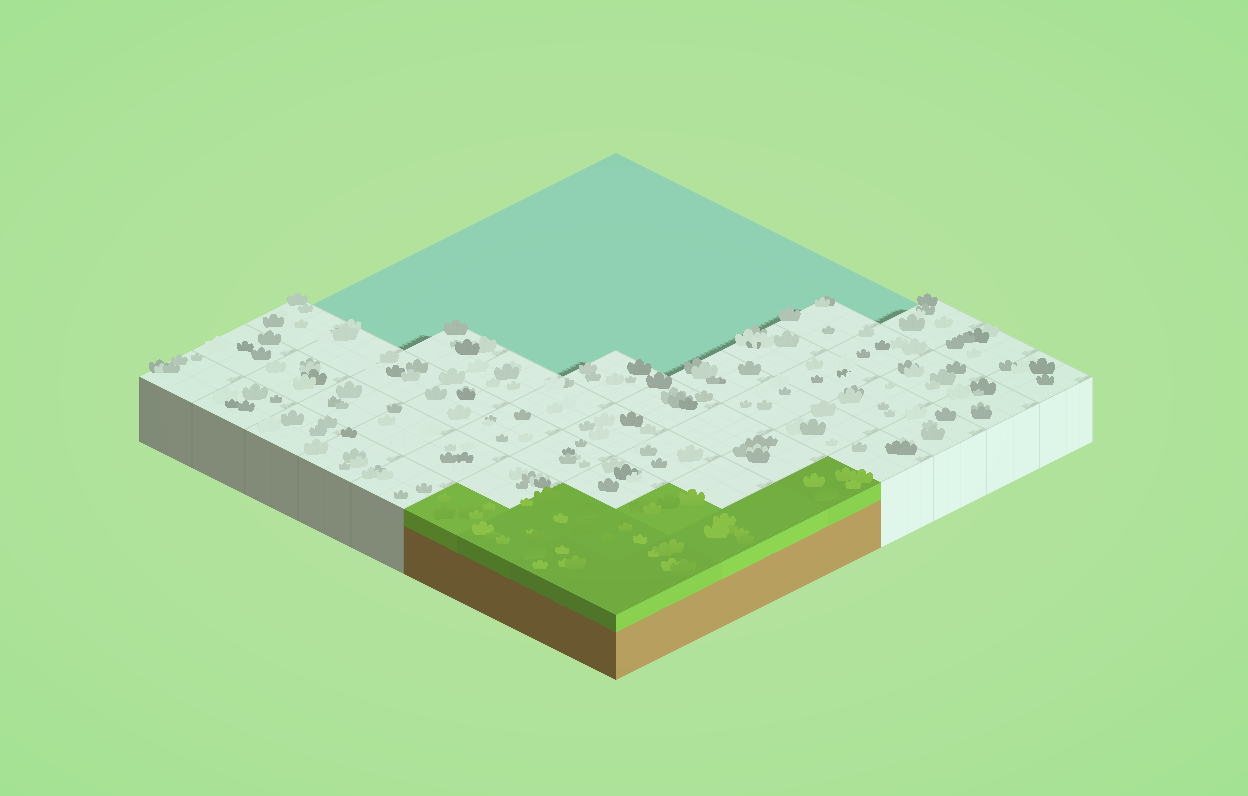
\includegraphics[width=350px,clip=true]{snaptogrid.png}
  \caption{Cuadrícula formada utilizando SnapToGrid}
  \label{fig:snaptogrid}
\end{figure}

\subsection{Generador de Mazmorras}
El generador de mazmorras está compuesto por dos componentes  que funcionan en tándem, por un lado existe la definición de tipos y algoritmos que permiten la construcción 
'teórica' de las mazmorras y laberintos, compuesto por clases y tipos como 'SquaredDungeon', 'Labyrinth' o 'Direction'. Estas clases (Figuras \ref{fig:dungen1} y \ref{fig:dungen2}) permiten generar una cuadrícula utilizando 
un array doble que posteriormente es poblado utilizando o bien el algoritmo de Prim (Código \ref{alg:dungenprim}) o Depth First Search, en adelante DFS (Código \ref{alg:dungendfs}). El sistema tiene la capacidad de transformar las matrices en grafos si es necesario, y es capaz de aplicarle a dichos grafos 
DFS o Breadth First Search para conseguir una lista de nodos en el orden indicado por el algoritmo.  

\begin{figure}[H]
  \centering
    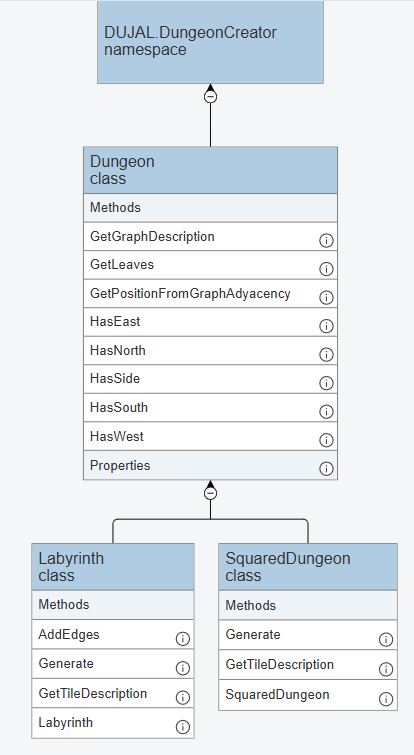
\includegraphics[width=200px,clip=true]{Dungeon_Generator.png}
  \caption{Diagrama Clases del Generador de Mazmorras}
  \label{fig:dungen1}
\end{figure}

\begin{figure}[H]
  \centering
    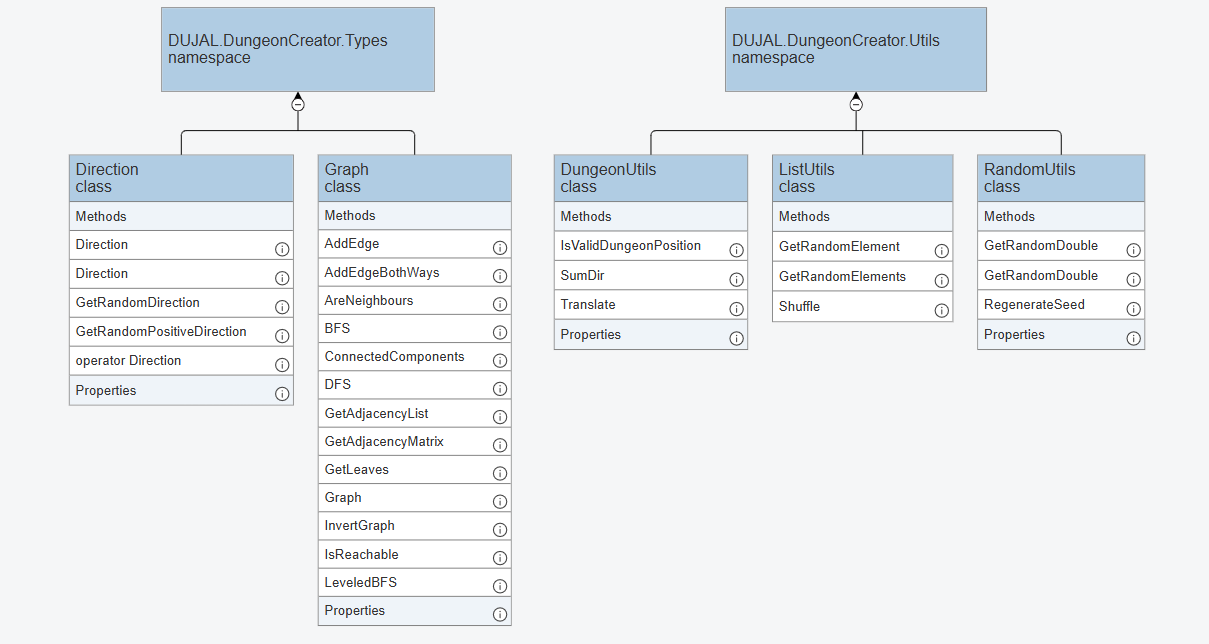
\includegraphics[width=450px,clip=true]{Dungeon_Generator_Utils.png}
  \caption{Diagrama Clases del Generador de Mazmorras}
  \label{fig:dungen2}
\end{figure}

\begin{mypython}[caption={Algoritmo de Generación de Mazmorras utilizando Prim.},label={alg:dungenprim}]
    protected void GeneratePrim(Vector2Int startingPos, int rooms = int.MaxValue)
    {
        PriorityQueue<Edge> edges = new();
        int num = 0;

        bool[,] visited = new bool[Size, Size];
        edges.Enqueue(new Edge(startingPos, startingPos + Direction.GetRandomPositiveDirection(), Random.Range(0, 10000)));
        edges.Enqueue(new Edge(startingPos, startingPos + Direction.GetRandomPositiveDirection(), Random.Range(0, 10000)));

        visited[startingPos.x, startingPos.y] = true;
        while (edges.Count() > 0 && num < rooms - 1)
        {

            Edge edge = edges.Dequeue();
            Vector2Int end = edge.end;
            Vector2Int origin = edge.origin;

            if (!visited[end.x, end.y])
            {
                visited[end.x, end.y] = true;
                _dungeonMatrix[end].Add(origin);
                _dungeonMatrix[origin].Add(end);
                ++num;

                for (Direction dir = 0; dir < Direction.Count; ++dir)
                {
                    Vector2Int newPos = end + dir.Vector;
                    if (DungeonUtils.IsValidDungeonPosition(newPos, Size))
                    {
                        edges.Enqueue(new Edge(end, newPos, Random.Range(0, 10000)));
                    }
                }
            }
        }
    }
\end{mypython}

\begin{mypython}[caption={Algoritmo de Generación de Mazmorras utilizando DFS.},label={alg:dungendfs}]
    protected void GenerateDFS(Vector2Int startingPos, int rooms = int.MaxValue)
    {
        int roomIdx = 0;
        Direction[,,] directionGrid = GenerateDFSDirectionGrid();

        bool[,] visited = new bool[Size, Size];

        Stack<int> roomStack = new();
        roomStack.Push(DungeonUtils.Translate(startingPos, Size));

        visited[startingPos.x, startingPos.y] = true;
        while (roomStack.Count > 0 && roomIdx < rooms)
        {
            Vector2Int roomPos = DungeonUtils.Translate(roomStack.Pop(), Size);
            for (Direction dir = 0; dir < Direction.Count; ++dir)
            {
                Vector2Int tentativePos = DungeonUtils.SumDir(directionGrid[roomPos.x, roomPos.y, dir], roomPos, Size);
                if (tentativePos != DungeonUtils.InvalidVector && !visited[tentativePos.x, tentativePos.y] && roomIdx < rooms)
                {
                    visited[tentativePos.x, tentativePos.y] = true;
                    roomStack.Push(DungeonUtils.Translate(tentativePos, Size));
                    _dungeonMatrix[roomPos].Add(tentativePos);
                    _dungeonMatrix[tentativePos].Add(roomPos);
                    ++roomIdx;
                }
            }
        }
    }
\end{mypython}

Una vez generada la mazmorra de forma teórica en formato mapa, es el turno de la parte dependiente del motor, que se encarga de instanciar 'GameObjects' de tipo 'DungeonRoom' 
basándose en la descripción de la matriz generada. Para ello la clase 'DungeonGenerator' tiene en si una lista de todas las permutaciones de sala posibles (Con puerta en cada 
posible lado entre norte, sur, este u oeste) y de todas los tipos de sala posibles (dados los tipos relevantes) para un juego o nivel concreto. Se busca una lista de 
'DungeonRooms' válidas para las coordenadas x, y que se quieran rellenar en un momento dado, y se selecciona una aleatoriamente para instanciar. Esto permite generar laberintos
y mazmorras como en los ejemplos de las Figuras \ref{fig:labyrinthExample} y \ref{fig:dungeonExample}.

\begin{figure}[H]
  \centering
    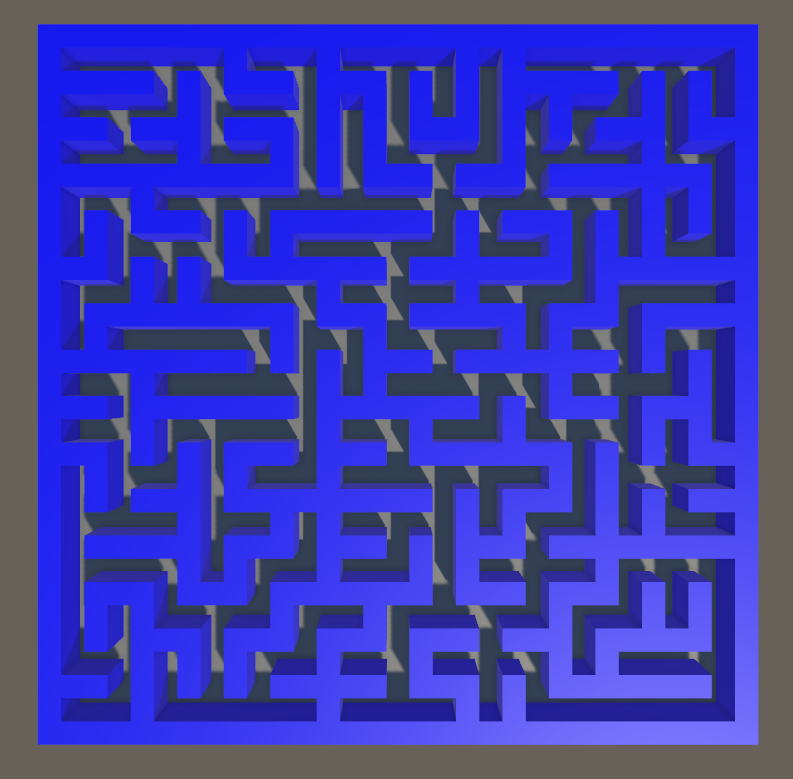
\includegraphics[width=350px,clip=true]{labyrinth_example.png}
  \caption{Laberinto Generado}
  \label{fig:labyrinthExample}
\end{figure}

\begin{figure}[H]
  \centering
    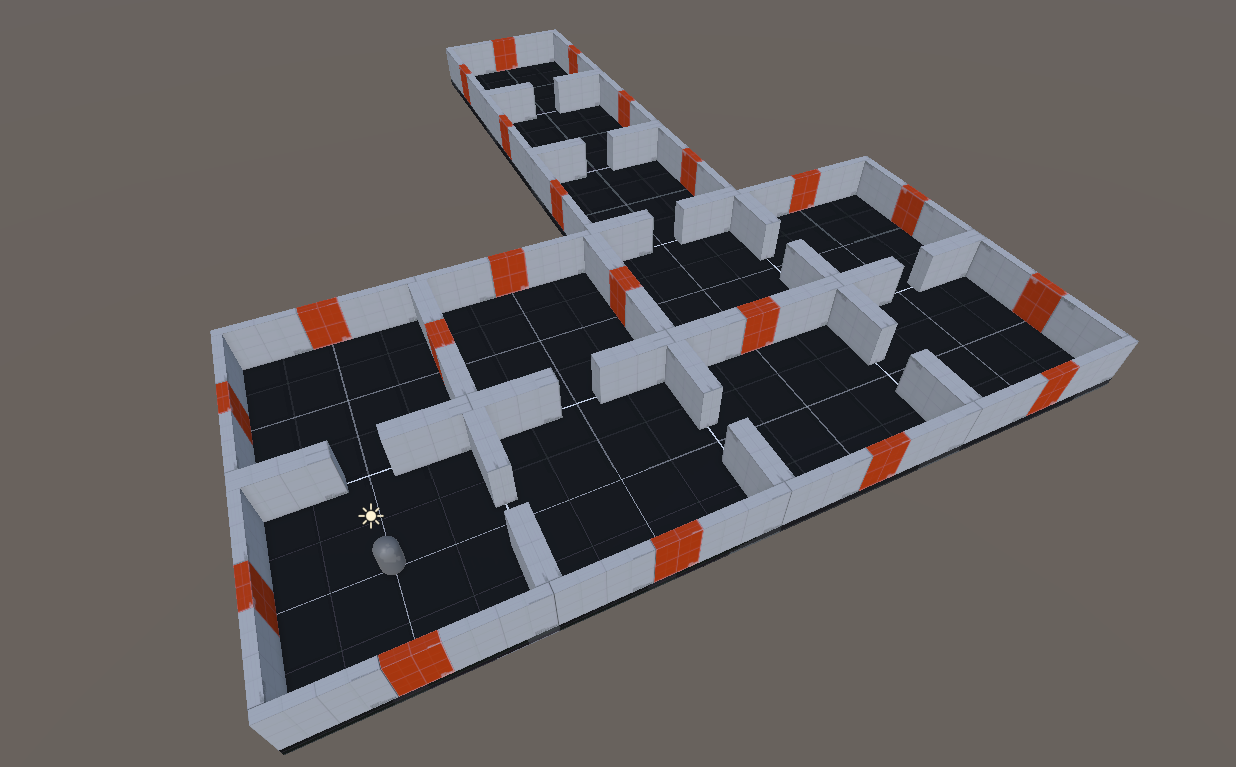
\includegraphics[width=350px,clip=true]{DungeonExample.png}
  \caption{Mazmorra Generada}
  \label{fig:dungeonExample}
\end{figure}

\subsection{Floater}
El componente de floater es una clase muy sencilla que permite darle a un objeto un movimiento de flotación sinuidal y de rotación constante dado un ángulo configurado. La 
implementación es muy sencilla dado que solo es necesario aplicarle un desplazamiento sinuidal en el bucle 'Update()' utilizando la diferencia de tiempo entre un ciclo y otro.

\begin{figure}[H]
  \centering
    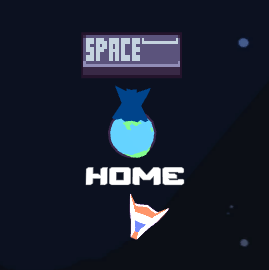
\includegraphics[width=200px,clip=true]{floaterExample.png}
  \caption{Ejemplo de uso de Floater, en el que el icono de 'Space' sube y baja para llamar la atención sobre el botón que debe presionar el jugador.}
  \label{fig:floaterExample}
\end{figure}


\subsection{Componente de Vida}
El componente de vida es un componente que se puede añadir a cualquier 'GameObject' y que permite atribuirle 'puntos de vida' a ese objeto. Aparte de métodos para acceder 
o modificar a la vida actual, también es posible añadir eventos para cuando el componente pierda vida, gane vida, cambie de vida, se quede sin vida o se cure completamente. 
Cabe destacar que el componente no es solamente útil para darle puntos de vida a un enemigo como se ha hecho tradicionalmente, sino que se podría utilizar, por ejemplo, 
para tener un callback concreto que disparar tras un temporizador, ya que podría deducirse un punto de vida por segundo.


\subsection{Componente de Interacción}
El componente de interacción permite añadir una callback a un 'UnityEvent' que se dispara cuando se pulsa el botón definido en el mapa de input correspondiente. 
Hay dos pares de clases 'Interactor', 2D y 3D, y dos pares de clases Interactable. Los interactors son las partes móviles, mientras que el interactable es el componente que 
tiene la callback asociada. Los interactables pueden configurarse para que solo se puedan usar una vez, se les puede configurar un radio de uso y se pueden deshabilitar. 
En el modo editor se puede pintar la esfera de radio que permite la interacción (Figura \ref{interactor}).

\begin{figure}[H]
  \centering
    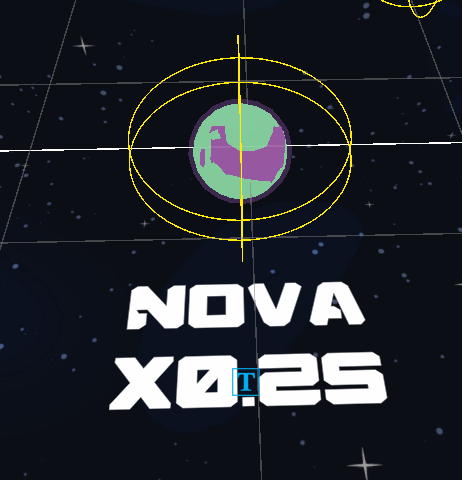
\includegraphics[width=200px,clip=true]{interactor.png}
  \caption{Radio de uso de un Interactor.}
  \label{fig:interactor}
\end{figure}

\subsection{LaunchRigidbody}
LaunchRigidbody es una clase pública y estática que no es un componente, al utilizar composición para funcionar no necesita existir en la escena, ya que recibe por parámetro 
el componente de Rigidbody que va a utilizar. La función además permite recibir dos 'Vector3' para indicar tanto la dirección como la potencia a la que se va a disparar el 
sólido rígido (Código \ref{alg:launchRigidbody}).

\begin{mypython}[caption={Funcionamiento de LaunchRigidbody.},label={alg:launchRigidbody}]
    public static void LaunchRigidBody3D(Rigidbody rigidbody, Vector3 launch, Vector3 power)
    {
        rigidbody.AddForce(new Vector3(launch.normalized.x * power.x, launch.normalized.y * power.y, launch.normalized.z * power.z), ForceMode.Impulse);
    }
\end{mypython}
    
\subsection{Componente de LookAtCamera}
Es un componente muy sencillo que rota un objeto en dirección a la 'Main Camera' (Código \ref{alg:alg:lookAtCamera}).

\begin{mypython}[caption={Funcionamiento de LookAtCamera.},label={alg:lookAtCamera}]
    var camera = Camera.main;
    transform.LookAt(transform.position + camera.transform.rotation * Vector3.forward, camera.transform.rotation * Vector3.up);
    transform.Rotate(_rotOffset);
\end{mypython}

\subsection{Componente de Sacudida de Cámara}
El componente de sacudida de cámara permite provocar un efecto de sacudida configurable de varias formas, aparte de definir la potencia y duración de la sacudida (Figura \ref{fig:screenshake2}), se puede 
estipular que la intensidad de la sacudida varíe en el tiempo utilizando una curva de animación (Figura \ref{fig:screenshake1}). Es relevante mencionar que hay dos variantes del componente, para cámaras 2D y 
cámaras 3D, como se menciona en la sección del estado del arte\ref{sec:estadodelarte}, en el estudio de Jump Trajectory\cite{Screenshake} se explica que la sacudida en 2D puede 
ser de traslación en los ejes XY ya que es como más se percibe el movimiento de la cámara en ese formato, pero que la sacudida en 3D debe ser por fuerza un movimiento 
exclusivamente rotatorio, ya que en caso contrario puede ocurrir clipping, además de que el movimiento de la cámara en esos casos es mucho más antinatural, ya que ninguna cámara
 en un espacio tridimensional puede trasladarse instantáneamente de esa forma. Cabe destacar también que el componente es capaz de funcionar con Cinemachine y cámaras normales. 

 
 \begin{figure}[H]
    \centering
    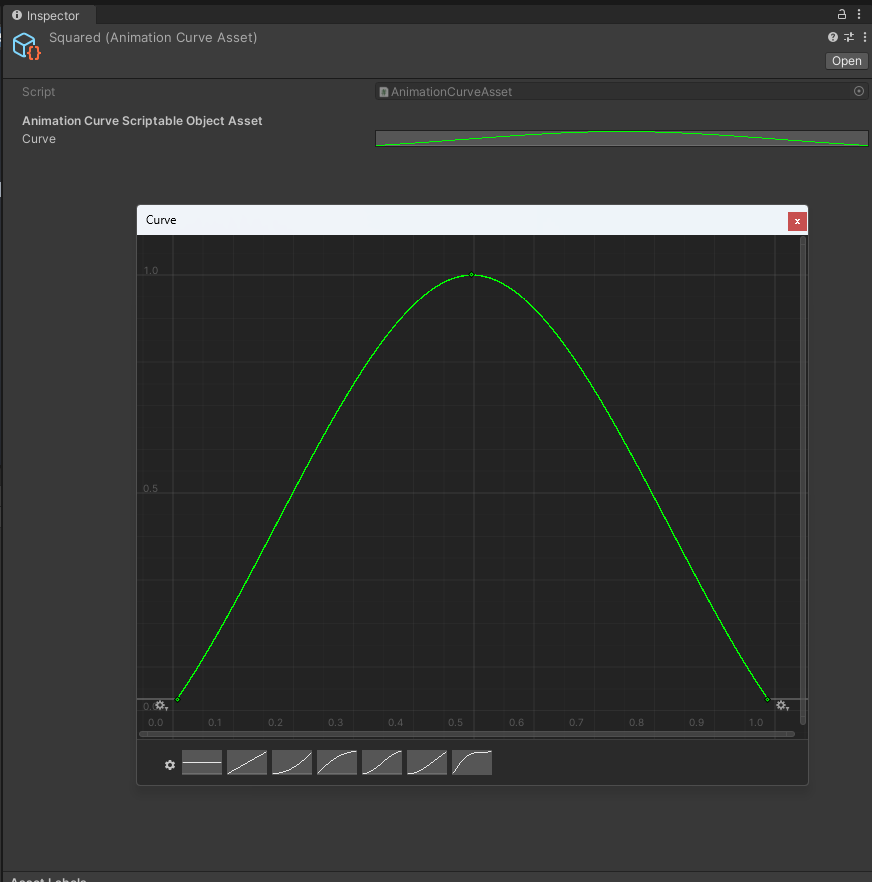
\includegraphics[width=350px,clip=true]{screenshakecurve.png}
    \caption{Configuración de Curva de Animación de Sacudida de Cámara.}
    \label{fig:screenshake1}
\end{figure}

\begin{figure}[H]
  \centering
    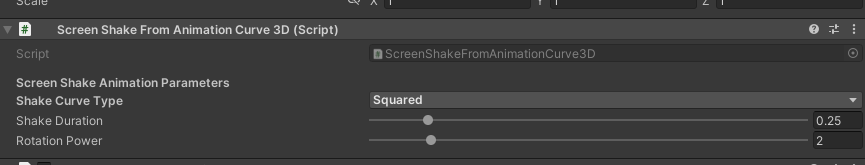
\includegraphics[width=350px,clip=true]{screenshake2.png}
  \caption{Configuración de Sacudida de Cámara.}
  \label{fig:screenshake2}
\end{figure}


\subsection{Componentes de Movimiento}
Los componentes de movimiento del paquete están todos basados en un componente del que heredan, el 'MovementComponent' (Figura \ref{fig:umlMovimiento}). Este 'MovementComponent' 
es útil para gestionar funcionalidades base de todos los componentes de movimiento, como habilitar o deshabilitar los controles o contener la referencia al gestor y mapa de input, 
también gestiona el cambio de mando a teclado y ratón y vice versa.

\begin{figure}[H]
  \centering
    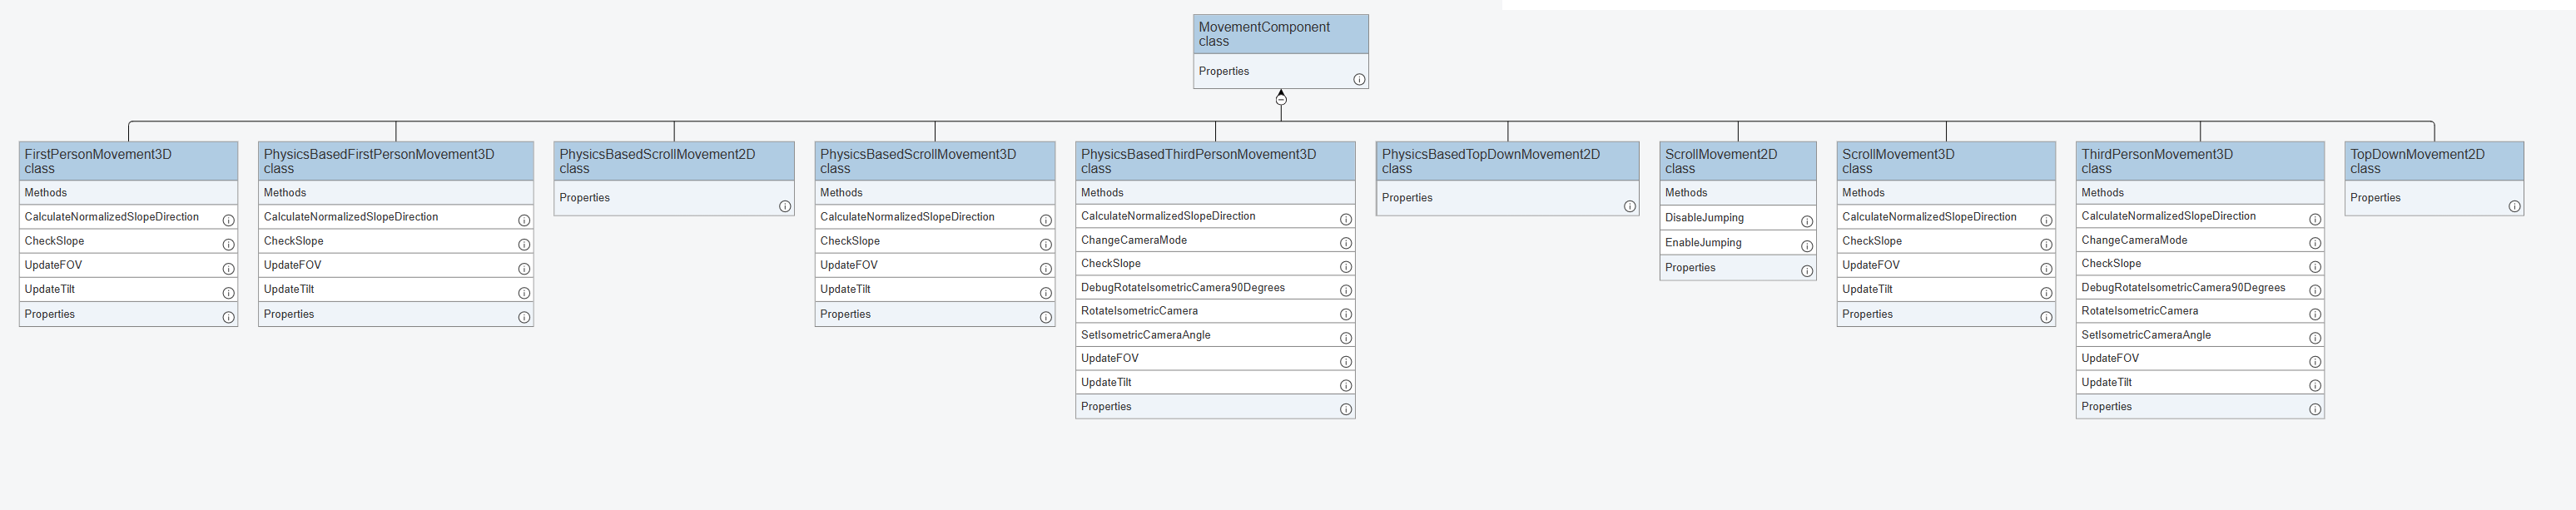
\includegraphics[width=350px,clip=true]{Movement.png}
  \caption{Diagrama de clases de los componentes de movimiento.}
  \label{fig:umlMovimiento}
\end{figure}

Aparte de los componentes de movimiento propios de cada cámara y si usan físicas o no, hay una clase 'CameraFollower' que gestiona las cámaras tridimensionales de Tercera Persona 
y Laterales. Esta clase gestiona sobre todo acompañar el movimiento del jugador, pudiendo configurarse para ajustar la suavidad con la que lo sigue, si alguno de los ejes 
es fijo, la zona muerta o si hay algún offset.

Otro dato relevante a nivel de arquitectura de software es que los componentes físicos se comportan como componentes auxiliares y externos, de forma que, por ejemplo,
 el PhysicsBasedFirstPersonMovement3D puede funcionar sin el componente de 'Wallrun' o el 'Dash', pero estos pueden añadirse al jugador tan solo con añadir el componente sin
 tener que hacer más ajustes.
 
Todos los componentes de movimiento funcionan con una máquina de estados que opera sobre el sólido rígido que constituye el cuerpo del jugador/personaje, y aplica distintas 
fuerzas a este dependiendo del input del jugador. El movimiento normal, por ejemplo, transforma el input de un joystick en dos ejes de \[-1,1\] a un vector director en el que 
aplicar la fuerza del movimiento. Por otra parte, agacharse implica forzar el estado a 'Crouching', bajar la cámara para ajustarse a la bajada de la cabeza del personaje, además de una reducción de velocidad y
un cambio en el FOV.

\section{Niveles de Prueba}
De acuerdo con los requisitos funcionales del proyecto, se ha desarrollado una serie de niveles de prueba para mostrar las distintas facetas de la suite de herramientas. En el proyecto de Unity, estos se encuentran
en la carpeta de Assets/TestScenes, y hay seis.

\subsection{2D Side Scroller Test Scene}
O y P para screen shake, WASD moverse, espacio saltar y wall jump. Collider 2D. Controller Side Scroll 2D, Camera Follower

\subsection{2D Top Down Test Scene}
Top Down Controller. Space Dash. E Interact. Camera Follow. Follow cursor rotation. Snap to Grid

\subsection{3D SideScroller + Dialogue}
Haz clic en 'Start Dialogue' para ver que tipo de cosas se pueden lograr con el sistema de diálogo. Hay un '3D Character Controller' que permite un scroll lateral tridimensional al acabar el diálogo. Hay 
dos controladores, uno basado en físicas y otro discreto.

\section{Documentación}


% Capítulo 4
\chapter{Validación}
\label{sec:validacion}

Para la validación del proyecto se ha distribuido el paquete de herramientas a varios equipos de desarrollo con el fin de encuestar a los distintos miembros acerca de la facilidad de uso, utilidad y escalabilidad.
 Entre estos equipos se encuentran los desarrolladores de Co-Fi Space\cite{CoFiSpace}, un videojuego de 'Game Jam' y EcoRescue\cite{EcoRescue} un trabajo de fin de grado, además de una serie de agentes 
 independientes que han prestado su tiempo a probar la librería en prototipos menores.

\section{Encuestas}

De cara a validar el proyecto, la primera fuente de datos planteada fue preparar una encuesta (Disponible en el Anexo \ref{sec:apendice}) con la que obtener sensaciones e impresiones de primera mano de los equipos
 de desarrollo y agentes individuales. El objetivo de estas preguntas es tanto obtener una idea general de si la 'suite' de herramientas es verdaderamente útil e intuitivo como si realmente es escalable como
 se pretendía en un principio.

\section{Experiencia de Validación}
La experiencia en general ha sido muy buena, el feedback ha sido en su mayoría positivo o en su defecto muy útil para seguir mejorando el proyecto a futuro. Los dos juegos que han resultado a raíz del proyecto 
tienen una calidad y acabado muy altos. Los encuestados se han mostrado en todo momento muy receptivos a participar en el proceso de explicación de los componentes de la librería, comunicando su opinión y 
proporcionando feedback significativo en todo momento. Finalmente se han encuestado a catorce usuarios de la librería entre los equipos de desarrollo y encuestados independientes.

\section{Resultados Cuantitativos}
En cuanto a la discusión de resultados, se pueden observar varios patrones muy evidentes, el primero y el más importante es que, en su grandísima mayoría (ver figuras en Apéndice \ref{sec:apendice}) los encuestados
se han mostrado positivos al ser preguntados acerca de la facilidad de uso e implementación de cada uno de los componentes o sistemas de la librería. Una notable excepción es la del generador de mazmorras, donde
 casi un 30\% (Figura \ref{fig:CUESTIONARIO_14trucado}) de los encuestados se han mostrado parcialmente o completamente en desacuerdo con que sea un sistema sencillo de utilizar, cabe destacar que esto es algo que 
 también se ha mencionado como feedback adicional (Figura \ref{fig:tablaFeedback}).

\begin{figure}[H]
  \centering
  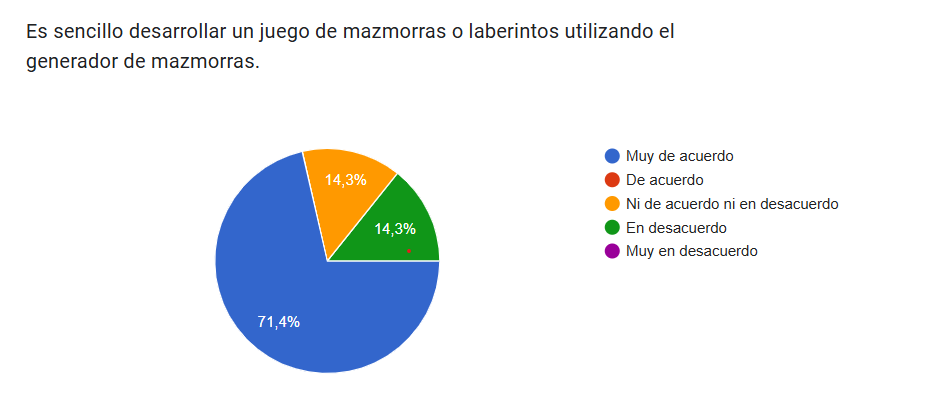
\includegraphics[width=450px,clip=true]{CUESTIONARIO_14.png}
  \caption{Encuesta sobre la facilidad de uso del sistema de mazmorras.}
  \label{fig:CUESTIONARIO_14trucado}
\end{figure}
\raggedbottom

Es relevante mencionar que a excepción del componente de sacudida de cámara, para el cual un 14\% (dos personas) (Figura \ref{fig:CUESTIONARIO_26trucado}) no han estado ni de acuerdo ni en desacuerdo, la totalidad de 
los encuestados están como mínimo parcialmente de acuerdo en que los 'Componentes Independientes' son fáciles de usar y se ajustan a sus respectivos casos de uso.

\begin{figure}[H]
  \centering
  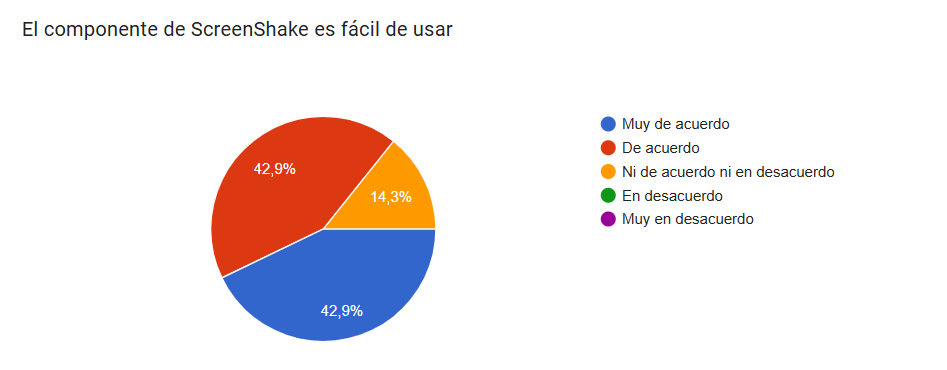
\includegraphics[width=450px,clip=true]{CUESTIONARIO_26.png}
  \caption{Encuesta sobre la facilidad de uso del componente de sacudida de cámara.}
  \label{fig:CUESTIONARIO_26trucado}
\end{figure}
\raggedbottom

La estadística puede parecer menos favorable en las preguntas que suelen hacer mención a la escalabilidad o sencillez del código de la librería, donde un 30\% de los encuestados opina que tanto el sistema de
 diálogo como el de audio son difíciles de escalar (Figuras \ref{fig:CUESTIONARIO_3trucado} y \ref{fig:CUESTIONARIO_6trucado}), o que un 60\% de los encuestados opina que la API del sistema de mazmorras es
  difícil de utilizar (Figura \ref{fig:CUESTIONARIO_15trucado}).Si bien es verdad que esta estadística cobra más sentido al tener en cuenta que el 30\% de los encuestados no tienen un perfil orientado a
   la programación (Figura \ref{fig:CUESTIONARIO_32trucado}), queda otro 30\% de programadores que aún así no opina que la API sea sencilla de utilizar. Una posible explicación al respecto, aparte de que quizás la
   documentación haya sido deficiente al respecto, como se menciona en la figura \ref{fig:tablaFeedback}, es que parte de la api del generador de mazmorras este exige al usuario un cierto
    conocimiento de algoritmos de recorrido de grafos y estructuras de datos complejas, que no todo el mundo, aun teniendo un perfil tecnológico, tiene necesariamente. 

\begin{figure}[H]
  \centering
  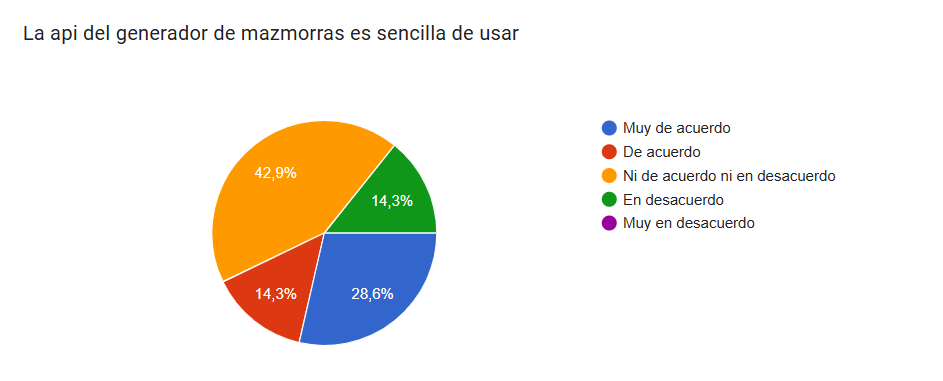
\includegraphics[width=450px,clip=true]{CUESTIONARIO_15.png}
  \caption{Encuesta sobre la sencillez del código del sistema de mazmorras.}
  \label{fig:CUESTIONARIO_15trucado}
\end{figure}
\raggedbottom

\begin{figure}[H]
  \centering
  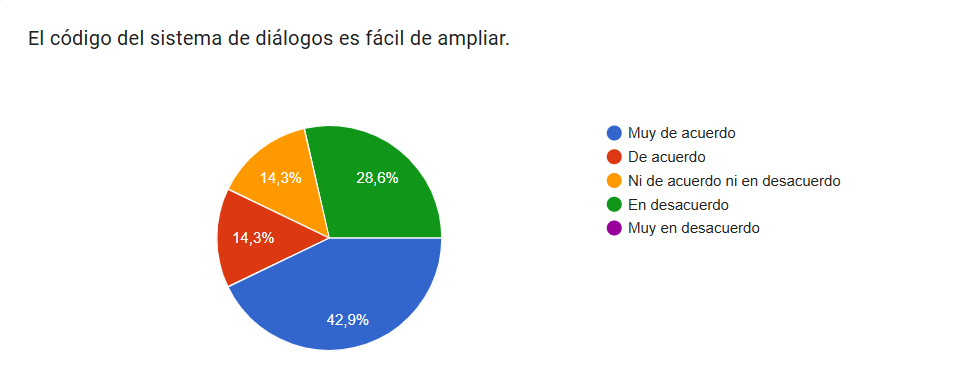
\includegraphics[width=450px,clip=true]{CUESTIONARIO_3.png}
  \caption{Encuesta sobre la escalabilidad del sistema de diálogo.}
  \label{fig:CUESTIONARIO_3trucado}
\end{figure}
\raggedbottom

\begin{figure}[H]
  \centering
  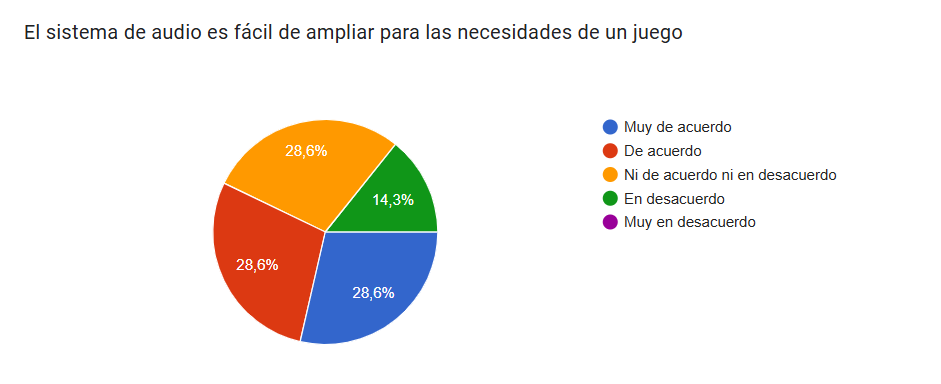
\includegraphics[width=450px,clip=true]{CUESTIONARIO_6.png}
  \caption{Encuesta sobre la escalabilidad del sistema de audio.}
  \label{fig:CUESTIONARIO_6trucado}
\end{figure}
\raggedbottom

\begin{figure}[H]
  \centering
  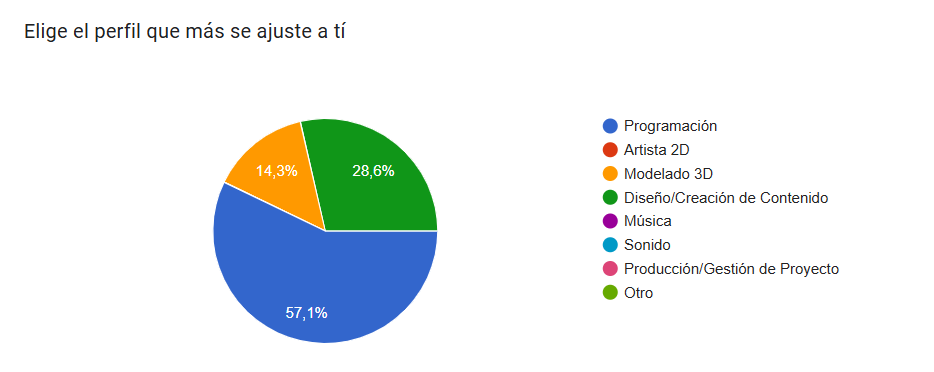
\includegraphics[width=450px,clip=true]{CUESTIONARIO_32.png}
  \caption{Encuesta sobre el perfil del encuestado.}
  \label{fig:CUESTIONARIO_32trucado}
\end{figure}
\raggedbottom

Como pequeños apuntes generales:
\begin{itemize}
    \item La gran mayoría de los encuestados opina que los componentes de movimiento y debug son útiles y efectivos.
    \item La media de edad de los encuestados ronda los veintiséis años de edad.
    \item Un 60\% de los encuestados tienen un perfil técnico, mientras que hay cuatro diseñadores y dos modeladores.
\end{itemize}

\section{Datos Cualitativos}
Hay que hacer énfasis en lo increíblemente participativos que se han mostrado los encuestados a la hora de trabajar en sus propios proyectos, todos los encuestados han usado la gran mayoría de sistemas que ofrecen
los distintos componentes de la libería, por enumerar ejemplos en los dos proyectos ya citados:
\begin{compactitem}
    \item Los niveles de cafetería en Co-Fi Space utilizan el sistema de experiencia.
    \item El movimiento en Co-Fi Space utiliza el componente de movimiento en tercera persona.
    \item El audio tanto en Co-Fi Space como en EcoRescue es gestionado por el sistema de audio.
    \item Los diálogos en ambos proyectos utilizan el sistema de diálogo.
    \item Los iconos de input y los componentes 2D de ambos proyectos utilizan los componentes de Floater y LookAtCamera.
    \item La cuadrícula de EcoRescue utiliza una versión modificada del componente SnapToGrid. 
\end{compactitem}

En cuanto al feedback proporcionado en la encuesta (Figura \ref{fig:tablaFeedback}), ya se ha mencionado que uno de los encuestados opinaba que la documentación es 'mejorable' y que otro de los encuestados opinaba 
que 'el generador de mazmorras es ligeramente complejo de usar sin un trasfondo ténico'. En esta útlima opinión parece estar de acuerdo otro encuestado, que mencionaba que 'algunas de las funcionalidades de la
 librería está muy orientadas a programadores, cosas como ampliar las animaciones de texto no son viables para alguiensin (o con pocos) conocimientos técnicos', sin embargo, tanto ese mismo encuestado como otros 
 cuantos más, coinciden en que 'en cuanto a las funcionalidades que norequieren programar, la librería resulta muy útil y dinámica para prototipar', que es una 'gran librería' y que 'lo demás (lo que no requiere
 implicación técnica) está muy guay'. Uno de los programadores añade incluso que desde el punto de vista técnico 'el código está muy bien comentado y es, por lo general, fácil de leer. Cabe destacar que el sistema de diálogo ha recibido buen feedback, este último programador opina que 'es sorprendente lo cómodo que se hace utilizar el sistema de diálogo', cosa que queda reflejada también
  en los resultados de las encuestas (Figuras \ref{fig:CUESTIONARIO_1} y \ref{fig:CUESTIONARIO_2}). El último punto de feedback indica que sería interesante que 'el componente SnapToGrid fuese aplicable al gameplay'
  esto es algo que, como se ha dicho en la lista anterior, ya se implementó para el videojuego EcoRescue, con lo cual la solución sería tan sencila como implementar los cambios que se ejecutaron para ese proyecto.

En cuanto a resultados tangibles del proyecto, es relevante mencionar que los dos proyectos formales que han sido desarrollados con esta librería han resultado rotundos éxitos. Co-Fi Space obtuvo una 6ª posición en 
la 'Game Jam' para la que fue presentado, y el trabajo de fin de grado EcoRescue obtuvo una calificación de nueve con ocho. 


% Capítulo 5

\chapter{Conclusiones y Trabajos Futuros}
\label{sec:conclusiones}

\section{Consecución de Objetivos}

Al inicio de este documento se enumeraba un resumen de los objetivos generales y secundarios de este proyecto, que incluían.

Principales:
En resumen, el el proyecto pretende, como objetivo principal desarrollar un paquete de herramientas completo y funcional que permita a los usuarios prototipar y 
 desarrollar videojuegos. Dicho paquete debe contener diversos sistemas y componentes 'prefabricados' que agilicen el desarrollo. 

\begin{compactitem}
    \item Desarrollar un paquete de herramientas completo y funcional.
    \item Dicho paquete debe permitir a los usuarios prototipar y desarrollar videojuegos.
    \item Tambén debe contener una serie de módulos divididos en: Sistemas Atómicos, Herramientas de Debug, Generador de Mazmorras, Componentes Independientes y Componentes de Movimiento de Personajes.
\end{compactitem}

Secundarios:
\begin{compactitem}
  \item Que los componentes del paquete sean escalables.
  \item Desarrollar niveles de prueba para servir a modo de tutorial para los usuarios.
  \item Documentar el modo de uso y funcionamiento de los componentes del proyecto.
  \item Validar el paquete con usuarios reales.
  \item Construir varios prototipos utilizando el paquete.
  \item Ajustar el paquete en base a los resultados de una encuesta de satisfacción.
\end{compactitem}

A continuación se discute el grado de consecución de cada objetivo:
\begin{enumerate}[itemsep=0mm]

\item Conclusion objetivo 1.
  
\item Conclusion objetivo 2.

\item Conclusion objetivo 3.

\end{enumerate}

\section{Trabajo Futuro}

De cara a futuras actualizaciones de DUJAL y teniendo en cuenta el feedback, habría que añadir una serie de mejoras: 
\begin{itemize}
    \item Mejora 1.
    \item Mejora 2.
    \item Mejora 3.
\end{itemize}

\section{Conclusiones Personales}
Personalmente opino que el proyecto ha sido un rotundo éxito, se ha desarrollado un paquete que a todas luces ha resultado verdaderamente útil de cara al prototipado de
 videojuegos con componentes que además de ser usables e intuitivos, el feedback ha demostrado que también son escalables. Además, a un nivel personal he aprendido mucho acerca
  de las tecnologías acerca que las que quería aprender, y estoy orgulloso del resultado tanto a nivel de usuario como con la complejidad técnica de la que se compone el proyecto. 

\blankpage


%%%%%%%%%%%%%%%%%%%%%%%%%%%%%%% Bibliografía %%%%%%%%%%%%%%%%%%%%%%%%%%%%%%%

\phantomsection
\addcontentsline{toc}{chapter}{Bibliografía}

\footnotesize{
%\bibliographystyle{hispa}
\bibliographystyle{IEEEtran}
\bibliography{bibliografia}
}



% No expandir elementos para llenar toda la página
\raggedbottom
\newpage

%%%%%%%%%%%%%%%%%%%%%%%%%%%%%%% Apéndices %%%%%%%%%%%%%%%%%%%%%%%%%%%%%%%

\appendix

\phantomsection
\addcontentsline{toc}{chapter}{Anexos}

\mbox{}
\vfill
\begin{center}
\begin{Huge}
\textbf{Apéndices}
\end{Huge}
\end{center}
\vfill
\mbox{}
\thispagestyle{empty}

\mbox{}
\thispagestyle{empty}


% Primer apéndice
\chapter{Anexo}
\label{sec:apendice}

\section{Documentos y Código}
\subsection{Documentación Técnica}

\href{https://github.com/dexaxi/RecursosSolarcore/blob/main/Assets/Documentation/Memoria%20-%20%C3%81ngel/tfg-template-master/EcoRescue.pdf}{Documentación}

\subsection{Repositorios}
\begin{itemize}
  \item DUJAL: \url{https://github.com/dexaxi/TFG_unity_package}
  \item UniTask: \url{https://github.com/Cysharp/UniTask}
\end{itemize}

\section{Tablas y figuras}

\subsection{Diagrama de Clases completo}

\begin{figure}[H]
  \centering
  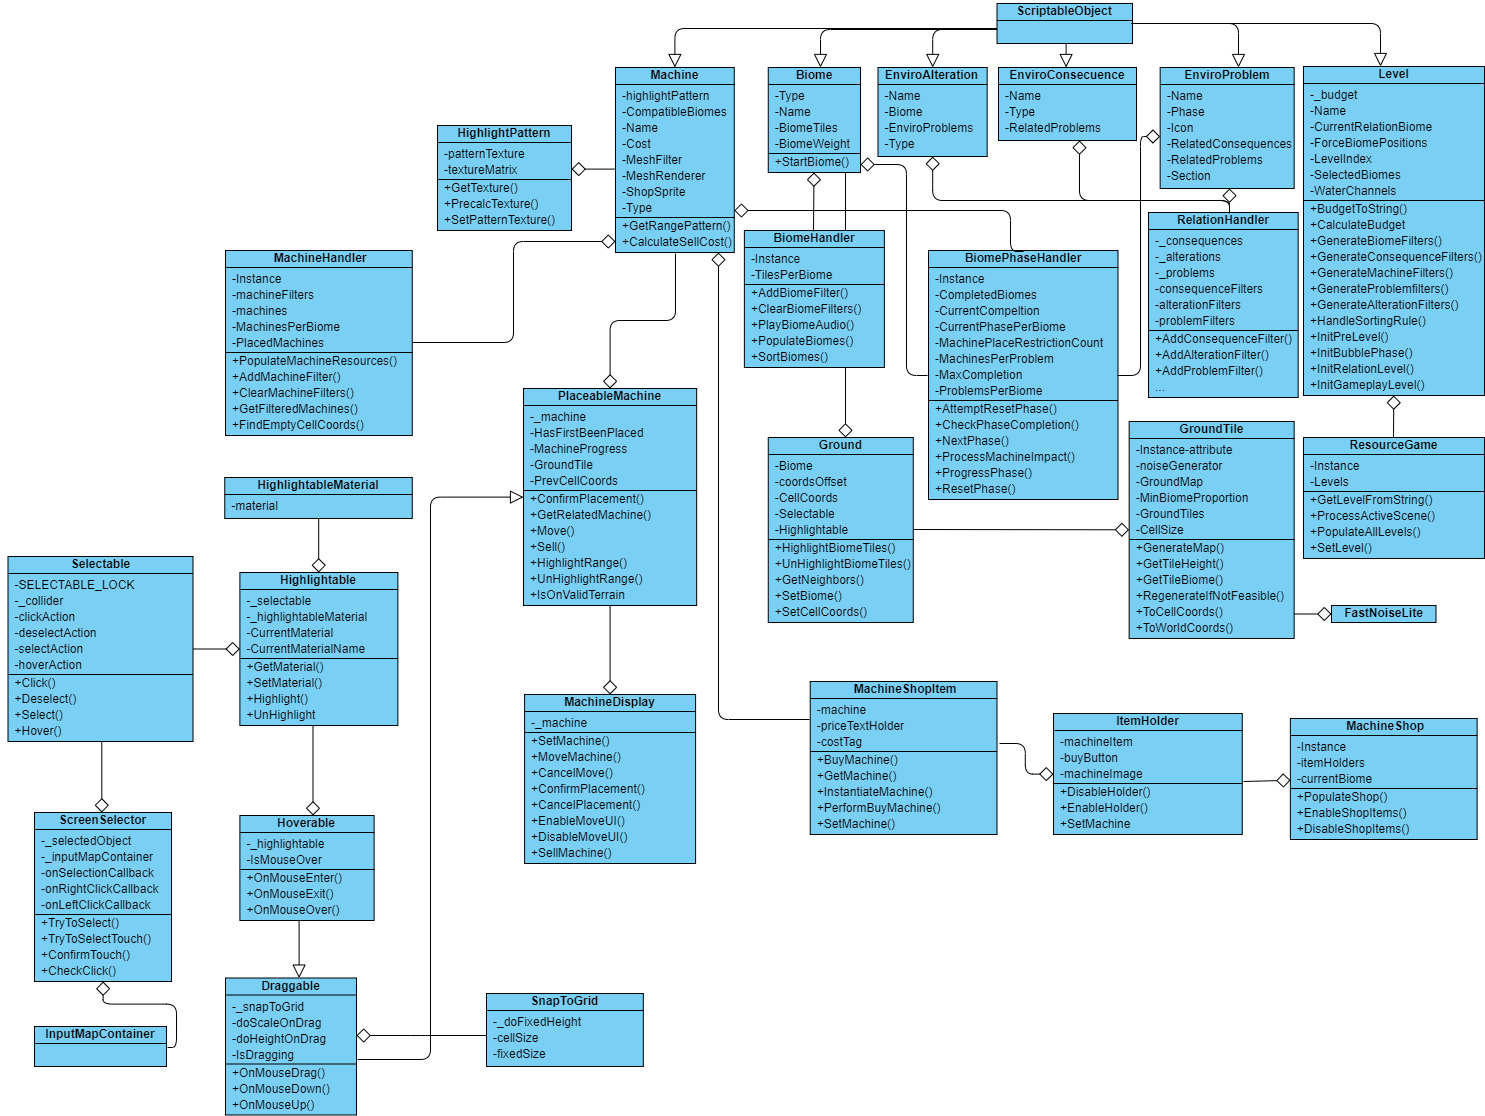
\includegraphics[width=450px,clip=true]{Logic_Class_Diagram.png}
  \caption{Diagrama de Clases completo}
  \label{fig:logicUML}
\end{figure}
\raggedbottom


\subsection{Resultados del Cuestionario}
% Insertar una figura
\begin{figure}[H]
  \centering
  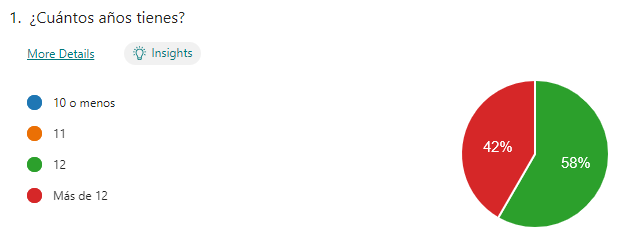
\includegraphics[width=450px,clip=true]{questionario_1.png}
  \caption{¿Cuántos años tienes?}
  \label{fig:questionario_1}
\end{figure}
\raggedbottom


% También con \pagebreak

% Fin del documento
\end{document}
